\documentclass[10pt]{article}

\addtolength{\topmargin}{-.5in}
\addtolength{\textheight}{1in}

\usepackage{amsmath}
\let\OldAngle\angle
\renewcommand{\angle}{\anglesym}

\usepackage{rotating}
\usepackage{graphicx}
\graphicspath{{figures/}}

\usepackage{epstopdf}
\epstopdfsetup{outdir=./}

\usepackage{natbib}
\bibpunct{[}{]}{;}{n}{,}{,} % required for natbib

\usepackage{multirow,tabularx}
% \usepackage{SIunits}
\usepackage{xspace}
\usepackage[table]{xcolor}% http://ctan.org/pkg/xcolor

\usepackage{hyperref}
\usepackage{hypcap} % Correct a problem with hyperref

\usepackage{circuitikz}
\usetikzlibrary{arrows}
\usepackage[justification=raggedright,font=small]{caption}
\usepackage{subcaption}

\usepackage{mathpazo}
\usepackage{lmodern,textcomp}

\usepackage{tcolorbox}% http://ctan.org/pkg/tcolorbox

\usepackage[free-standing-units]{siunitx}
\usepackage{cleveref}% load last



% \sisetup{math-degree=\mbox{\textdegree},text-degree=\textdegree}
% \sisetup{math-celsius=\mbox{\textdegree}C,text-celsius=\textdegree C}


\usepackage{mathtools}

\crefname{equation}{equation}{eq. }
\Crefname{equation}{Eq.}{Eq.}% For beginning \Cref
\crefrangelabelformat{equation}{(#3#1#4--#5#2#6)}

\crefmultiformat{equation}{eq. #2#1#3}{, #2#1#3}{#2#1#3}{#2#1#3}
\Crefmultiformat{equation}{Eq. #2#1#3}{, #2#1#3}{#2#1#3}{#2#1#3}

%\usepackage{pdfcomment}

% PDFCOMMENT EXAMPLES:

% You can do much more \pdfmarkupcomment[markup=Squiggly,color=green,author=CAP]{with pdfcomment}{move to the front}.
% This is a \pdfmarkupcomment[markup=StrikeOut,color=red,author=CAP]{stupid}{replace stupid with funny}  game!
% \pdfmarkupcomment[markup=Highlight,color=yellow,author=CAP]{Of course, you can highlight complete sentences.}{Highlight}
% This is very\pdfcomment[icon=Note,color=blue]{insert graphic!} interesting!

\newcommand{\specialcell}[2][c]{%
  \begin{tabular}[#1]{@{}l@{}}#2\end{tabular}}

\newcommand\redbox[3][red]{\textcolor{#1}{\rule{#2}{#3}}}

\newcommand{\brieftbllink}[1]{\hyperref[#1]{Tbl.~\ref*{#1}}\xspace }
\newcommand{\briefeqlink}[1]{\hyperref[#1]{Eq.~\ref*{#1}}\xspace }
\newcommand{\tablelink}[1]{\hyperref[#1]{Tbl.~\ref*{#1}}\xspace }
\newcommand{\eqlink}[1]{\hyperref[#1]{Equation~\ref*{#1}}\xspace }
\newcommand{\briefseclink}[1]{\hyperref[#1]{Sec.~\ref*{#1}}}
\newcommand{\briefappxlink}[1]{\hyperref[#1]{App.~\ref*{#1}}}
\newcommand{\seclink}[1]{\hyperref[#1]{Section~\ref*{#1}}}
\newcommand{\parbreak}{\ \\
\noindent}
\newcommand{\brieffiglink}[1]{\hyperref[#1]{Fig.~\ref*{#1}}}
\newcommand{\brieffigsublink}[2]{\hyperref[#1]{Fig.~\ref*{#1}#2}}

\newcommand{\vulgaronehalf}{${}^1\!\!\mskip0.3\thinmuskip/\!{}_2$}

\def\changemargin#1#2{\list{}{\rightmargin#2\leftmargin#1}\item[]}
\let\endchangemargin=\endlist 

\title{Practical Measurement of Voltage-Controlled Current Source Output Impedance for Applications in Transcranial Electrical Stimulation\\[.5cm]\colorbox{yellow!30}{\emph{Unabridged preprint}}\\[.1cm]\colorbox{yellow!30}{\small For the original paper and citation, please see Appendix}}

\author{Charl Linssen\\
\small Donders Institute for Brain, Cognition and Behaviour\\
\small Radboud University\\
\small Nijmegen, The Netherlands\\
\small \texttt{<c.linssen@donders.ru.nl>}\\[0.5cm]
Pieter Harpe\\
\small Integrated Circuits Group\\
\small Eindhoven University of Technology\\
\small Eindhoven, The Netherlands\\
\small \texttt{<p.j.a.harpe@tue.nl>}\\[0.5cm]
\date{\today}
}

%%%%%%%%%%%%%%%%%%%%%%%%%%%%%%%%%%%%%%%%%%%%%%%%%%%%%%%%%%%%%%%%%%%%%%%%%%%%%%
%%%%%%%%%%%%%%%%%%%%%%%%%%%%%%%%%%%%%%%%%%%%%%%%%%%%%%%%%%%%%%%%%%%%%%%%%%%%%%
\begin{document}

\maketitle

%%%%%%%%%%%%%%%%%%%%%%%%%%%%%%%%%%%%%%%%%%%%%%%%%%%%%%%%%%%%%%%%%%%%%%%%%%%%%%
%%%%%%%%%%%%%%%%%%%%%%%%%%%%%%%%%%%%%%%%%%%%%%%%%%%%%%%%%%%%%%%%%%%%%%%%%%%%%%
\begin{abstract}
\noindent A voltage-controlled current source (VCCS) is a key component in the electrical stimulation of neuronal tissue. We present a method for the evaluation of output impedance across frequency, of VCCS circuits with applications in transcranial electrical stimulation (tES). Two VCCS circuit architectures, one with a single-ended, and one with a differential output, are theoretically analysed and simulated, and the method is validated by matching these results with empirical measurements. Monte Carlo simulation of the measurement method itself is used to predict its range of applicability under real-world conditions. Both circuits, as well as the method used to determine output impedance, are easy to reproduce, using generic hardware components at low cost. The method described has immediate practical application value in neuroscience research, where it can be used in the deployment and further development of VCCS circuit architectures.
\end{abstract}

\tableofcontents


%%%%%%%%%%%%%%%%%%%%%%%%%%%%%%%%%%%%%%%%%%%%%%%%%%%%%%%%%%%%%%%%%%%%%%%%%%%%%%
\section{Motivation}
\label{sec:motivation}
%%%%%%%%%%%%%%%%%%%%%%%%%%%%%%%%%%%%%%%%%%%%%%%%%%%%%%%%%%%%%%%%%%%%%%%%%%%%%%

Transcranial electrical stimulation (tES) is a relatively non-invasive way of altering the excitability of the brain. A direct, alternating or noise current (tDCS, tACS or tRNS, respectively) is delivered between two electrodes that have been placed into conductive contact with the subject's skin, on or near the scalp (\brieffiglink{fig:situation_sketch}, top). Bandwidth of the stimulation is typically below $1~\kilo\hertz$ and currents are below $2~\milli\ampere$ \cite{pmid26652115}\cite{pmid19109497}. In addition to tES, voltage-controlled current sources are key components in other stimulation methods of the nervous system, such as Deep Brain Stimulation (DBS), where similar operating parameters are required \cite{dbs}.

\begin{figure}[bt]
	\begin{subfigure}{\textwidth}
        \centering
\makebox[\textwidth][c]{%
		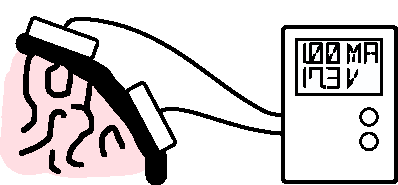
\includegraphics[scale=1.1]{fig_situation_sketch.pdf}
        % \caption{\small abc}
        }
        \caption{}
        \label{fig:situation_sketch1}
    \end{subfigure}

	\begin{subfigure}{\textwidth}
        \centering
\makebox[\textwidth][c]{%
\begin{circuitikz}
	\node [] (topleft) at (-1, 1) {};
	\node [] (bottomleft) at (-1, -1) {};

	\node [] (topright) at (2, 1) {};
	\node [] (bottomright) at (2, -1) {};

	\node [] (topright1) at (4, 1) {};
	\node [] (bottomright1) at (4, -1) {};

	\node [] (topright2) at (5, 1) {};
	\node [] (bottomright2) at (5, -1) {};

	\draw (topleft.center) to [generic, l=$Z_L$]  (bottomleft.center) {};
	\draw (bottomright1.center) to [generic, l=$Z_{out}$, *-*]  (topright1.center) {};
	\draw (bottomright2.center) to [american controlled current source, l_=$g_m$]  (topright2.center) {};
	\draw (topleft.center) to [generic, l=$Z_{elec}$, i<^=$I_L$]  (topright.center) {};
	\draw (bottomleft.center) to [generic, l=$Z_{elec}$]  (bottomright.center) {};
	\draw (topright.center) to [short] (topright1.center) {};
	\draw (bottomright.center) to [short] (bottomright1.center) {};
	\draw (topright1.center) to [short] (topright2.center) {};
	\draw (bottomright1.center) to [short] (bottomright2.center) {};

	%
	% 	RC poles: box
	%

	\node [] (vboxtr) at (2.75, 1.4) {};
	\node [] (vboxbr) at (2.75, -1.4) {};
	\node [] (vboxtl) at (6.25, 1.4) {};
	\node [] (vboxbl) at (6.25, -1.4) {};

	\draw[dashed] (vboxtr.center) to [short] (vboxbr.center) {};
	\draw[dashed] (vboxbr.center) to [short] (vboxbl.center) {};
	\draw[dashed] (vboxbl.center) to [short] (vboxtl.center) {};
	\draw[dashed] (vboxtl.center) to [short] (vboxtr.center) {};
\end{circuitikz}

}
        \caption*{\small}
        \label{fig:situation_sketch2}
    \end{subfigure}
\caption{\small Situation sketch (top panel) and equivalent circuit (bottom panel). In a typical tES session, the device is adjusted to supply a given current $I_L$ into a load $Z_L$ via two electrodes, each with interfacial impedance $Z_{elec}$. We assume the device is battery powered or in any case galvanically isolated; the ground node is thus elided in the bottom panel.}
\label{fig:situation_sketch}
\end{figure}

There is a trend towards smaller electrodes in tES, which allow for controlling the stimulation at a higher spatial resolution \cite{pmid23031743}. Smaller electrodes have a higher electrode (electrode/electrolyte, or interfacial) impedance (\brieffiglink{fig:situation_sketch}, bottom), and thus in general need higher drive voltages to maintain the same current. Drive voltages can also be paradoxically high, even with common tES electrode sizes (on the order of $50~\centi\meter^2$), for especially \emph{low} currents. For tDCS at $2.5~\milli\ampere$, an extrapolated voltage swing of at least $18.3~\volt$ is required from the VCCS, ``for the top 99th percentile'' of subjects \cite{pmid25018056}; \cite{pmid20488204} report using values as high as $66.7~\volt$.

To obtain larger output voltage swing, a VCCS with a differential output can be used. In a single-ended architecture, one of the electrodes is connected to ground, while the other is driven by the VCCS. In a differential design, instead, both sides are actively driven by the VCCS. This requires twice as many amplifiers or output drivers, but results in an effective doubling of the output voltage range when one side of the load is driven in antiphase with the other. Further benefits include an improved signal bandwidth, immunity to changes in the load, and noise immunity \cite{pmid24880419}.

Here, we present a universal, low-cost method to measure VCCS output impedance, to guide the design and empirical performance validation of any single-ended or differential output current source, in the operating regime that is typical for tES with human subjects. To improve the interpretability of obtained results, we selected two related circuits for evaluation, so that results may be compared on a relative basis. Each of these circuits is a variant of the well-known ``improved Howland'' current source, which can be built using commodity, off-the-shelf parts with low total cost, excellent performance, and large output voltage swing \cite{Franco1988}. Howland sources require precise matching of resistor values to obtain good performance, which can be adequately addressed by trimming using a single potentiometer (or two in the case of the differential source). These features make them an excellent alternative to custom silicon where access to tooling, turnaround time, customisation or cost are of concern.

We begin with a mathematical analysis (\briefseclink{sec:analysis}) and simulation studies (\briefseclink{sec:sim_results}), continue with empirical measurements (\briefseclink{sec:empirical-results}), and conclude in \briefseclink{sec:conclusion}.

\raggedbottom


%%%%%%%%%%%%%%%%%%%%%%%%%%%%%%%%%%%%%%%%%%%%%%%%%%%%%%%%%%%%%%%%%%%%%%%%%%%%%%
\section{Previous work}
\label{sec:previous_work}
%%%%%%%%%%%%%%%%%%%%%%%%%%%%%%%%%%%%%%%%%%%%%%%%%%%%%%%%%%%%%%%%%%%%%%%%%%%%%%

A straightforward differential version of the Howland current source uses two of the exact same single-ended Howland current sources, one to drive the anode and one to drive the cathode. A common drive signal (the voltage indicating current setpoint) is connected to the positive-phase input of the anodal VCCS and the negative-phase input of the cathodal VCCS \cite{1742-6596-407-1-012030}\cite{pmid19706961}. This configuration relies on the non-ideal (finite) output resistance of each current source to balance the two legs of the circuit, making it extremely sensitive to small variations in component values, causing an unacceptably large common-mode voltage.

A potential solution to the problem of imbalance is to use an active feedback circuit that nulls the common-mode voltage at the output \cite{US2002060915A1:misc}. This prevents one of the legs from floating to the supply rail. A disadvantage of this circuit is the large number of components used (7 op-amps and 14 precision resistors) and required matching.

The differential source in \cite{pmid24880419} is based on the single-ended improved Howland, but extends the circuit by two op-amps. A single-ended Howland source drives the anodal leg of the circuit as normal. A new pair of op-amps, configured as an inverting voltage follower, drive the cathode voltage to be equal and opposite to the anode voltage. This architecture was found to perform well in comparison to a normal, single-ended configuration, approximately doubling the differential output impedance over a wide frequeny range. This design shows a differential but not symmetric output, which could affect noise rejection to external interference, because the cathode terminal output impedance will be different from the anode terminal output impedance. Frequency compensation of the voltage follower can introduce additional instabilities.

Another family of circuits is based around the use of a fully differential output op-amp \cite{offsetfree_bidirectional_current_source}\cite{SirtoliMorcellesVincence}, which have the advantage of very small common-mode output voltage.

A fully differential circuit similar to the improved Howland was described in \cite{simmonds2009differential}. One op-amp is connected to the anode of the load through a sense resistor, and a second op-amp connects to the cathode through a second sense resistor. The net negative feedback to one op-amp is then given by the voltage drop over the sense resistor on the opposite leg. This circuit is fully symmetrical and requires only two standard op-amps and six precision resistors. In the remainder of this paper, we use this circuit as a benchmark.


%%%%%%%%%%%%%%%%%%%%%%%%%%%%%%%%%%%%%%%%%%%%%%%%%%%%%%%%%%%%%%%%%%%%%%%%%%%%%%
%%%%%%%%%%%%%%%%%%%%%%%%%%%%%%%%%%%%%%%%%%%%%%%%%%%%%%%%%%%%%%%%%%%%%%%%%%%%%%
\section{Analysis}
\label{sec:analysis}
%%%%%%%%%%%%%%%%%%%%%%%%%%%%%%%%%%%%%%%%%%%%%%%%%%%%%%%%%%%%%%%%%%%%%%%%%%%%%%

Throughout the analysis and results sections, we compare a single-ended with a differential VCCS using a common set of measurements. This allows us to distinguish the relative performance gained by changing to a differential architecture from the absolute performance, which is affected by implementation details such as selection of the op-amp IC.

In this section, we analytically determine the gain, compliance voltage and predicted output resistance for the single-ended version, followed by the differential circuit. Derivations were carried out with the help of Wolfram Mathematica \cite{mathematica}.


%%%%%%%%%%%%%%%%%%%%%%%%%%%%%%%%%%%%%%%%%%%%%%%%%%%%%%%%%%%%%%%%%%%%%%%%%%%%%%
\subsection{Single-ended ``improved'' Howland VCCS}
\label{sec:single_ended_howland}

The improved Howland circuit is based on a standard op-amp and five precision resistors. It is a single-ended circuit, meaning one side of the load is connected to ground (\brieffiglink{fig:single_ended_howland}). The operation of the circuit can be understood as follows: there is both negative feedback (via $R_2$) and positive feedback (via $R_{4a}$). The difference between positive and negative feedback is proportional to the load current (via the ratio $R_2/R_{4b}$). No current flows into the input terminals of the op-amp, so the same difference in current exists between $R_1$ and $R_3$. But as $V_{pos}=V_{neg}$ in normal operation, these currents are in turn proportional to the input voltage $V_{in,pos}-V_{in,neg}$. Thus, overall, the load current is proportional to the input voltage.


%%%%%%%%%%%%%%%%%%%%%%%%%%%%%%%%%%%%%%%%%%%%%%%%%%%%%%%%%%%%%%%%%%%%%%%%%%%%%%
\subsubsection{DC analysis}

\begin{figure}
\centering
\begin{circuitikz}

	\node [op amp] (opamp) {} (0,0);

	\node [label=left:$V_{in,pos}$] (Vinpos) at (-6, -2) {};
	\node [label=left:$V_{in,neg}$] (Vinneg) at (-6, 2) {};
	\node [label=below:$V_{pos}$] (op_vp) at (-2, -2) {};
	\node [label=above:$V_{neg}$] (op_vn) at (-2, 2) {};
	\node [label=right:$V_L$] (vb) at (2, -2) {};
	\node [label=right:$V_o$] (va) at (2, 0) {};
	\node [] (vdummy) at (2, -2.5) {};

	\draw (vb.center)+(0, -0.2) to [generic, l=$Z_L$, i>^=$I_L$] +(0, -2.2) node [rground] at +(0, -2) {};
	\draw (opamp.out) -- (va.center) {};

	\draw (Vinneg.center) to [R, l=$R_1$, o-*] (op_vn.center) {};
	\draw (Vinpos.center) to [R, l=$R_3$, o-*] (op_vp.center) {};
	\draw (op_vp.center) to [R, l=$R_{4a}$] (vb.center) {};
	\draw (va.center) |- (2, 2) to [R, l_=$R_2$] (op_vn.center) {};
	\draw (vb.center) -- (vdummy.center) {};

	\draw (opamp.+) -| (-2, -2) to (op_vp.center) {};
	\draw (opamp.-) -| (-2, 2) to (op_vn.center) {};

	\draw (va) to [R, l^=$R_{4b}$, *-o] (vb) {};
\end{circuitikz}

\caption{\small Circuit diagram of the single-ended ``improved'' Howland source. $Z_L$ is the load impedance external to the VCCS.}
\label{fig:single_ended_howland}
\end{figure}

Let $A_{OL}$ be the (finite) gain of the op-amp. The input-output relationship of the op-amp can be written as
\begin{subequations}
\label{eq:prerequisites}
\begin{gather}
\label{eq:finite_gain_opamp}
V_o = A_{OL}\cdot(V_{pos}-V_{neg})\\
\intertext{To derive the gain of the VCCS, we start by applying Kirchhoff's Current Law (KCL) to node $V_{pos}$ and $V_{neg}$:}
\label{eq:finite_gain_opamp2}
\frac{V_{in,pos}-V_{pos}}{R_3} - \frac{V_{pos} - V_L}{R_{4a}}=0\\
\frac{V_o - V_{neg}}{R_2} - \frac{V_{neg} - V_{in,neg}}{R_1}=0\\
\intertext{Similarly we apply KCL to the output node $V_L$:}
\frac{V_o-V_L}{R_{4b}} + \frac{V_{pos}-V_L}{R_{4a}} - I_L = 0\label{eq:se_1}
\end{gather}
\end{subequations}
For a given load $Z_L$, and assuming $A_{OL}=\infty$, combining \briefeqlink{eq:finite_gain_opamp}---\briefeqlink{eq:se_1} yields the transfer function of the VCCS:
\begin{align}
\label{eq:single_ended_howland_transfer_function}
\frac{I_L}{V_{in,diff}} = \frac{1}{2}\cdot\frac{R_2 (R_3 + 2 R_{4a}) + R_1(R_{4a} + R_{4b})}{R_2 R_3 Z_L - R_1 (R_3 R_{4b} + R_{4b} Z_L + R_{4a} (R_{4b} + Z_L))}
\end{align}
with $V_{in,diff}=V_{in,pos}-V_{in,neg}$. Under the conditions that
\begin{subequations}
\label{eq:single_ended_howland_conditions}
\begin{align}
A_{OL} &= \infty\\
R_1 &= R_3\label{eq:single_ended_howland_conditions_r1}\\
R_2 &= R_{4a} + R_{4b}\label{eq:single_ended_howland_conditions_r2}
\end{align}
\end{subequations}
\briefeqlink{eq:finite_gain_opamp}---\briefeqlink{eq:se_1} simplify such that the output current does not depend on output voltage (i.e. the $V_L$-dependent term vanishes). The transfer function can then be written as:
\begin{subequations}
\label{eq:single_ended_gain}
\begin{equation}
I_L = g_m\cdot V_{in,diff}
\end{equation}
with
\begin{equation}
g_m = \frac{R_2}{R_3R_{4b}}
\end{equation}
\end{subequations}
the transconductance of the VCCS in units of Amp\`{e}re per Volt.

%%%%%%%%%%%%%%%%%%%%%%%%%%%%%%%%%%%%%%%%%%%%%%%%%%%%%%%%%%%%%%%%%%%%%%%%%%%%%%
\subsubsection{Output resistance}
\label{sec:singla_ended_output_resistance}

Ideally, the output resistance of a VCCS is infinite. In practice, it attains only a finite value, due to limitations of the op-amp, and imperfect matching of the resistors (violations of \briefeqlink{eq:single_ended_howland_conditions} and \briefeqlink{eq:diff_howland_conditions}). An expression for output impedance can be obtained by taking the partial differential of the output voltage with respect to the output current:
\begin{align}
\label{eq:rout_single_ended}
Z_{out} &= \frac{\partial V_L}{\partial{}I_L}\nonumber\\
&= -\frac{\alpha + A_{OL}\cdot\beta}{\gamma + A_{OL}\cdot\delta}
\end{align}
with
\begin{align}
\alpha &= (R_1 + R_2) (R_3 + R_{4a}) R_{4b}\nonumber\\
\beta &= R_1 (R_3 + R_{4a}) R_{4b}\nonumber\\
\gamma &= (R_1 + R_2) (R_3 + R_{4a} + R_{4b})\nonumber\\
\delta &= R_1 (R_{4a} + R_{4b}) - R_2 R_3\nonumber
\end{align}
which is indeed infinite under the conditions given by \briefeqlink{eq:single_ended_howland_conditions}.

Note that for certain combinations of values, the output resistance can exhibit a negative sign. In this case, load current will increase with increasing load resistance. Intuitively, it is a consequence of the positive feedback in the circuit (via $R_{4a}$) being too strong with respect to the negative feedback (via $R_2$). This situation, where positive feedback dominates, could theoretically cause instability. The magnitude of the effect is in the form of a transconductance with magnitude (``differential gain'') equal to $1/|Z_{out}|$. Thus, for a circuit where the resistors are reasonably well matched, $Z_{out}$ is very high and this gain is infinitessimal.

%  if the load exhibits a nonlinearity, for example, if $R_L$ itself decreases with voltage $V_L$.


%%%%%%%%%%%%%%%%%%%%%%%%%%%%%%%%%%%%%%%%%%%%%%%%%%%%%%%%%%%%%%%%%%%%%%%%%%%%%%
\subsubsection{Compliance voltage}
\label{sec:single_ended_compliance_voltage}

The compliance voltage (maximum output voltage span) is in practice limited by the saturation voltage of the op-amp $V_{sat,pp}$ (e.g. $28~\volt$ for a $\pm15~\volt$ op-amp), and the voltage drop across the series resistor $R_{4b}$ caused by $I_L$, while the contribution of the positive feedback path (through $R_{4a}$) is negligible:

\begin{align}
\label{eq:single_ended_compliance_voltage}
|V_L|\leq V_{sat,pp} - R_{4b}|I_{L,max}|
\end{align}
To obtain the largest output voltage swing, $R_{4b}$ should be chosen as small as possible, taking other constraints on the circuit into account.






\begin{figure}[tb]
\centering
\noindent\makebox[\textwidth]{%
\begin{circuitikz}
	\node [op amp] (opampa) at (0, -3) {} (0, 0);
	\node [op amp, yscale=-1] (opampb) at (0, 3) {} (6, 6);

	\node [ocirc, label=left:$V_{in,neg}$] (Vinpos) at (-3., -3.5) {};
	\node [ocirc, label=left:$V_{in,pos}$] (Vinneg) at (-3., 3.5) {};
	\node [circ, label=left:\raisebox{-0.9cm}{$V_{a,neg}$}] (VAneg) at (1.75, .75) {};
	\node [circ, label=left:\raisebox{0.8cm}{$V_{b,neg}$}] (VBneg) at (1.75, -.75) {};
	\node (VAneg2) at (4, -.75) {};
	\node (VBneg2) at (4, .75) {};
	\node [label=above:$V_a$] (VA) at (1.75, 3.) {};
	\node [label=below:$V_b$] (VB) at (1.75, -3.) {};

	\node (VLposint) at (4., 3.) {};
	\node (VLnegint) at (4., -3.) {};
	\node [] (von2) at (4.75, -0.75) {};
	\node [label=above:$V_{L,pos}$] (vlpos) at (6.75, 3) {};
	\node [label=below:$V_{L,neg}$] (vlneg) at (6.75, -3) {};

	\draw (VB.center) to [R, l^=$R_{4b}$, *-*] (VLnegint.center) {};
	\draw (VA.center) to [R, l^=$R_{2b}$, *-*] (VLposint.center) {};

	\draw (Vinpos.center) to [o-] (opampa.+) {};
	\draw (Vinneg.center) to [o-] (opampb.+) {};

	\draw (opampb.-) |- (VAneg) {};
	\draw (opampa.-) |- (VBneg) {};
	\draw (opampa.out) -- (VB.center) {};
	\draw (opampb.out) -- (VA.center) {};
	\draw (VAneg.center) -- (VAneg2.center) to [R, label=$R_{4a}$] (VLnegint.center) {};
	\draw (VLposint.center) to [R, label=$R_{2a}$] (VBneg2.center) -- (VBneg.center) {};
	\draw (VBneg.center) to [R, l=$R_3$] (VB.center) {};
	\draw (VA.center) to [R, l=$R_1$] (VAneg.center) {};

	\draw (VLposint.center) -- (vlpos.center) to [generic, l=$Z_L$, i>^=$I_L$, o-o] (vlneg.center) -- (VLnegint.center) {};
\end{circuitikz}

}
\caption{\small Circuit diagram of the fully differental ``improved'' Howland source. $Z_L$ is the load impedance external to the VCCS.}
\label{fig:differential_howland}
\end{figure}




%%%%%%%%%%%%%%%%%%%%%%%%%%%%%%%%%%%%%%%%%%%%%%%%%%%%%%%%%%%%%%%%%%%%%%%%%%%%%%%
%%%%%%%%%%%%%%%%%%%%%%%%%%%%%%%%%%%%%%%%%%%%%%%%%%%%%%%%%%%%%%%%%%%%%%%%%%%%%%%
\subsection{Differential version of the ``improved'' Howland VCCS}
\label{sec:differential_howland}

To actively drive both sides of the load, the differential version uses two op-amps and six precision resistors (\brieffiglink{fig:differential_howland}). It operates in a manner analogous to the single-ended version, the voltages in the bottom half having equal magnitude but opposite sign from the top half at all times. For each of the halves, the positive part of the feedback is now obtained via the negative input terminal of the op-amp. This is achieved by obtaining the feedback voltage from the other side of the circuit, where it has an inverted sign (this is the X-shaped crossing in the circuit). $R_1$ and $R_3$ in the differential circuit are analog to $R_2$ in the single-ended version, conveying negative feedback. $R_{2a}$ and $R_{4a}$ are analogous to $R_{4a}$ in the single-ended circuit and convey what is effectively positive feedback because of the sign inversion.

%%%%%%%%%%%%%%%%%%%%%%%%%%%%%%%%%%%%%%%%%%%%%%%%%%%%%%%%%%%%%%%%%%%%%%%%%%%%%%%
\subsubsection{DC analysis}

Starting again with the definition of an op-amp with finite gain $A_{OL}$:
\begin{subequations}
\label{eq:diff_1}
\begin{gather}
V_a = A_{OL}\cdot(V_{in,pos} - V_{a,neg})\\
V_b = A_{OL}\cdot(V_{in,neg} - V_{b,neg})
\end{gather}
\end{subequations}
Apply KCL to nodes $V_{L,pos}$ and $V_{L,neg}$:
\begin{subequations}
\label{eq:diff_2}
\begin{gather}
\frac{V_a - V_{L,pos}}{R_{2b}} - \frac{V_{L,pos} - V_{b,neg}}{R_{2a}} - I_L = 0\\
\frac{V_b - V_{L,neg}}{R_{4b}} - \frac{V_{L,neg} - V_{a,neg}}{R_{4a}} + I_L = 0
\end{gather}
\end{subequations}
Apply KCL to nodes $V_{a,neg}$ and $V_{b,neg}$:
\begin{subequations}
\label{eq:diff_3}
\begin{gather}
\frac{V_a - V_{a,neg}}{R_1} + \frac{V_{L,neg} - V_{a,neg}}{R_{4a}} = 0\\
\frac{V_b - V_{b,neg}}{R_3} + \frac{V_{L,pos} - V_{b,neg}}{R_{2a}} = 0
\end{gather}
\end{subequations}
In addition, we use the auxilary equation for the differential output voltage $V_L$:
\begin{equation}
\label{eq:diff_4}
V_L = V_{L,pos} - V_{L,neg}
\end{equation}
For a given load $Z_L$, and assuming $A_{OL}=\infty$, combining \briefeqlink{eq:diff_1}--\briefeqlink{eq:diff_4} yields the transfer function:
\begin{align}
\label{eq:diff_howland_transfer_function}
\frac{I_L}{V_{in,diff}} = \frac{R_1 (R_{2a} + R_3) + R_{4a} (R_{2a} + R_3) - R_{2b} R_{4b} }{ \left( \begin{aligned}&Z_L((R_{2a} + R_{2b})(R_{4a} + R_{4b}) - R_1 R_3)\\&+ R_{2a}(R_{4b}(R_1 + R_{4a}) + R_{2b}(R_{4a}+R_{4b}))\\&+ R_{2b}R_{4a}(R_3+R_{4b})\end{aligned}\right)}
\end{align}
Under the conditions that
\begin{subequations}
\label{eq:diff_howland_conditions}
\begin{align}
R_{2b} &= R_{4b}\\
R_{2a} &= R_{4a}\\
R_1 = R_3 &= R_{2b} + R_{2a}\\
V_{in,pos} &= -V_{in,neg}
\end{align}
\end{subequations}
\briefeqlink{eq:diff_1}--\briefeqlink{eq:diff_4} simplify such that the output current does not depend on output voltage (i.e. the $V_L$ term vanishes). The transfer function can then be written as:
\begin{subequations}
\label{eq:diff_gain}
\begin{equation}
I_L = g_m \cdot V_{in,diff}
\end{equation}
with
\begin{equation}
g_m = \frac{1}{R_{2b}}
\end{equation}
\end{subequations}


%%%%%%%%%%%%%%%%%%%%%%%%%%%%%%%%%%%%%%%%%%%%%%%%%%%%%%%%%%%%%%%%%%%%%%%%%%%%%%%
\subsubsection{Compliance voltage}

The main limiting factor of the compliance voltage is, as before, the saturation voltage of the op-amp, and secondly, the voltage drop across (in this case not one but two) resistors $R_{2b}$ and $R_{4b}$ (with $R_{2b}=R_{4b}$). If resistor values are chosen to be equal (see \tablelink{tbl:resistor_vales}), this yields a compliance voltage twice that of the single-ended variant:
\begin{align}
\label{eq:diff_compliance_voltage}
|V_L|\leq 2\left(V_{sat,pp} - R_{2b}|I_{L,max}|\right)
\end{align}


%%%%%%%%%%%%%%%%%%%%%%%%%%%%%%%%%%%%%%%%%%%%%%%%%%%%%%%%%%%%%%%%%%%%%%%%%%%%%%%
\subsubsection{Output resistance}
\label{sec:symmetrical_vccs_output_resistance}

The differential output resistance:
\begin{align}
\label{eq:rout_diff}
R_{out} &= \frac{\partial V_L}{\partial{}I_L}\nonumber\\
&= \frac{\alpha + A_{OL}\cdot\beta}{\gamma + A_{OL}\cdot\delta}
\end{align}
with
\begin{align}
\alpha &= (R_{4b} + R_{4a} + R_1) (R_{2b} + R_{2a} + R_3)\nonumber\\
\beta &= (R_{2b} + R_{2a})(R_{4b} + R_{4a}) - R_1 R_3\nonumber\\
\gamma &= R_{4b} (R_{4a} + R_1) (R_{2a} + R_3)\nonumber\\
&\ \ \ \ \ \ \ + R_{2b} ((R_{4a} + R_1) (R_{2a} + R_3) + R_{4b} (R_{4a} + R_{2a} + R_1 + R_3))\nonumber\\
\delta &= R_{4b} R_{2a} (R_{4a} + R_1) + R_{2b} (R_{4b} (R_{4a} + R_{2a}) + R_{4a} (R_{2a} + R_3))\nonumber
\end{align}
which is indeed infinite under the conditions given by \briefeqlink{eq:diff_howland_conditions} and $A_{OL}=\infty$.




%%%%%%%%%%%%%%%%%%%%%%%%%%%%%%%%%%%%%%%%%%%%%%%%%%%%%%%%%%%%%%%%%%%%%%%%%%%%%%%
%%%%%%%%%%%%%%%%%%%%%%%%%%%%%%%%%%%%%%%%%%%%%%%%%%%%%%%%%%%%%%%%%%%%%%%%%%%%%%%
\section{Simulation results}
\label{sec:sim_results}

%%%%%%%%%%%%%%%%%%%%%%%%%%%%%%%%%%%%%%%%%%%%%%%%%%%%%%%%%%%%%%%%%%%%%%%%%%%%%%%
\subsection{Monte Carlo simulation of DC output resistance}
\label{sec:monte_carlo}

\begin{table}[t!]
\centering
\bgroup
\def\arraystretch{1.3}%  1 is the default, change whatever you need
\begin{tabularx}{.4\textwidth}{ X|X }
\multicolumn{2}{ c }{\large Single-ended}\\
\hline
 \cellcolor{gray!4} $R_1$, $R_2$, $R_3$ & \cellcolor{gray!4} $10.25~\kilo\ohm$\\
 \cellcolor{gray!8} $R_{4a}$ & \cellcolor{gray!8} $10~\kilo\ohm$\\
 \cellcolor{gray!4} $R_{4b}$ &  \cellcolor{gray!4} $250~\ohm$\\
\end{tabularx}\quad\begin{tabularx}{.4\textwidth}{ X|X }
\multicolumn{2}{ c }{\large Differential}\\
\hline
\cellcolor{gray!4} $R_1$, $R_3$ & \cellcolor{gray!4} $10.25~\kilo\ohm$\\
\cellcolor{gray!8} $R_{2a}$, $R_{4a}$ & \cellcolor{gray!8} $10~\kilo\ohm$\\
\cellcolor{gray!4} $R_{2b}$, $R_{4b}$ & \cellcolor{gray!4} $250~\ohm$\\
\end{tabularx}
\egroup
\caption{Component values used in all simulations and prototypes. The given combinations of values result in a gain $A=4~\milli\ampere/\volt$ for both circuits.}
\label{tbl:resistor_vales}
\end{table}

\begin{figure}[b!]
        \centering
        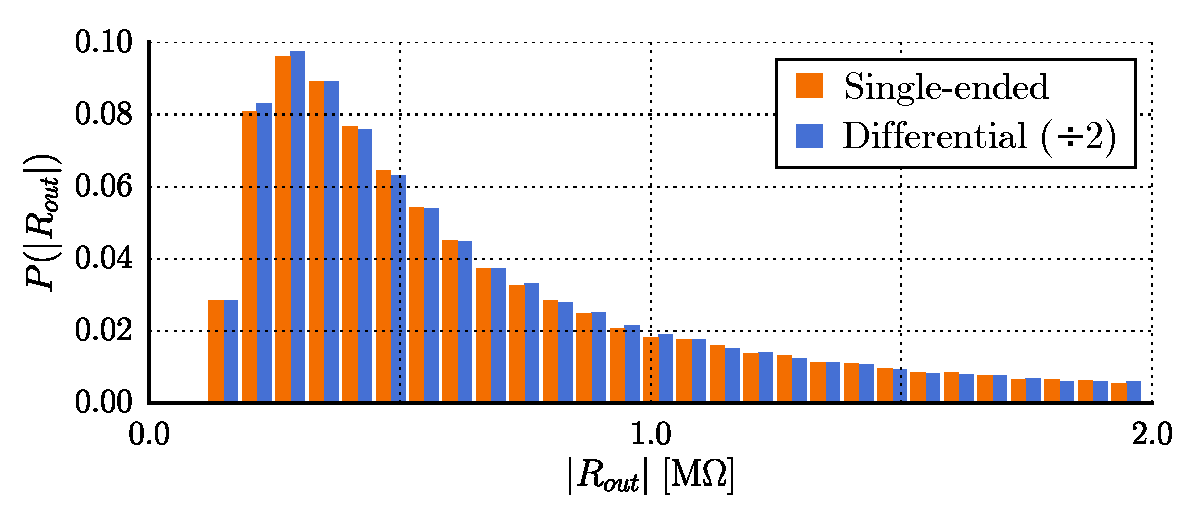
\includegraphics[scale=.6]{fig_mc_output_resistance.pdf}
        \caption{\small Monte Carlo simulation of absolute single-ended and differential DC output resistance for a resistor tolerance of 0.1\% and $A_{OL}=\infty$. For each VCCS type, $10^5$ samples were generated and it was assumed in both cases that the op-amp gain $A_{OL}=\infty$. Note that the output resistance of the differential VCCS is twice as high as the single-ended VCCS but is scaled by a factor \textonehalf~in this plot to allow easier visual comparison.}
        \label{fig:mc_output_resistance}
\end{figure}

To compare the output resistance attainable by both designs, we run a Monte Carlo simulation of the effect of mismatches. For each iteration of the Monte Carlo algorithm, we sample resistance values for all resistors in the circuit from a uniform distribution, centered upon a mean and within a 0.1\% tolerance range. The mean value for each resistor is given in \tablelink{tbl:resistor_vales}; these values are consistently used throughout simulations and prototyping. After sampling, output resistance is calculated according to \briefeqlink{eq:rout_single_ended} (single-ended) or \briefeqlink{eq:rout_diff} (differential). The open-loop gain of all op-amps is here assumed to be infinite ($A_{OL}=\infty$).

For approximately half of the resistor value permutations, the sign of the output resistance is positive, while in the other half it is negative (see discussion in \briefseclink{sec:singla_ended_output_resistance}). The resulting distribution is symmetric around 0. To allow for a more concise plot, we consider only the absolute value $|R_{out}|$.

A histogram of attained output resistance is plotted in \brieffiglink{fig:mc_output_resistance}. For ease of visual comparison, the output resistance of the differential VCCS is scaled by a factor \textonehalf. The distributions for the single-ended and (scaled) differential output resistance are almost indistinguishable, demonstrating that for the same tolerance rating of the resistors, output resistance of the differential supply will be expected to be twice as high as that of the single-ended supply.

%%%%%%%%%%%%%%%%%%%%%%%%%%%%%%%%%%%%%%%%%%%%%%%%%%%%%%%%%%%%%%%%%%%%%%%%%%%%%%
\subsubsection{Tradeoff between VCCS gain and output impedance}
\label{sec:tradeoff_gain_impedance}

\begin{figure}[b!]
	\centering
	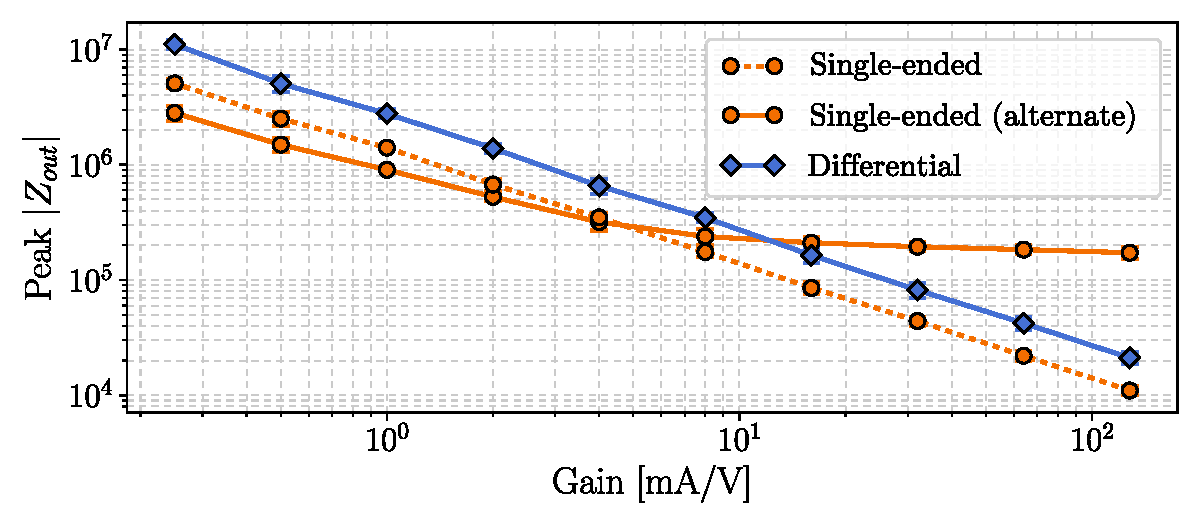
\includegraphics[scale=.6]{fig_mc_output_resistance_across_gain.pdf}
	\caption{\small A doubling of VCCS gain reduces the attained output impedance by half. Vertical axis shows the location of the peak of the distribution in \brieffiglink{fig:mc_output_resistance} for different values of VCCS gain (horizontal axis). The base values were picked for a gain of $4~\milli\ampere/V$.}
	\label{fig:mc_output_resistance_across_gain}
\end{figure}

Although it is not immediately clear from comparing the expressions for gain and output impedance (\briefeqlink{eq:single_ended_gain} and \briefeqlink{eq:rout_single_ended} for single-ended; \briefeqlink{eq:diff_gain} and \briefeqlink{eq:rout_diff} for differential), there is a negative relationship between achieved output impedance and VCCS gain. This can easily be demonstrated numerically, by running the Monte Carlo script of \brieffiglink{fig:mc_output_resistance} for different values of gain, and measuring the location of the peak of the distribution. The resulting plot illustrates the tradeoff between gain and output impedance (\brieffiglink{fig:mc_output_resistance_across_gain}). In the differential VCCS, gain can only be changed by changing the value of $R_{2b}$, so only one line is shown (blue diamonds). For the single-ended VCCS, gain can be changed in different ways: by changing the value of $R_3$ (orange circles, continuous line), or the value of $R_{4b}$ (orange circles, dashed line).

In all further simulations and experiments, we use a constant set of resistor values (\tablelink{tbl:resistor_vales}) to obtain a gain of $4~\milli\ampere/\volt$ for each VCCS, which yields practical voltage levels and places us in the middle range of the curves in \brieffiglink{fig:mc_output_resistance_across_gain}.



%%%%%%%%%%%%%%%%%%%%%%%%%%%%%%%%%%%%%%%%%%%%%%%%%%%%%%%%%%%%%%%%%%%%%%%%%%%%%%
\subsection{A practical method for measuring output impedance}
\label{sec:output_impedance_measurement}

The output impedance of a current source can be measured by the following method \cite{pmid24880419}. A voltage $V_{in,dif\!f}$ is applied to the VCCS corresponding to a current of $1~\milli\ampere$ AC peak, that is, $I_L=1~\milli\ampere\,\cdot\,\sin(2\pi{}ft)$. We then measure the load voltage $V_L=V_{L,pos}-V_{L,neg}$ and actual current delivered to the load $I_L$, under two conditions. Initially, a load $R_{L,a}$ is connected (\brieffiglink{fig:impedance_measurement_method}). The corresponding load voltage and current are denoted $V_{L,a}$ and $I_{L,a}$, respectively. The load is then changed to $R_{L,b}$, and again the load voltage $V_{L,b}$ and current $I_{L,b}$ are measured. The output impedance $Z_{out}$ can then be derived by circuit analysis:
\begin{subequations}
\label{eq:z_out}
\begin{align}
Z_{out} &= \frac{R_{L,a} R_{L,b} (V_{L,b} - V_{L,a})} {V_{L,a}R_{L,b} - V_{L,b} R_{L,a}} \label{eq:z_out_volt} \\
& = \frac{I_{L,b} R_{L,b} - I_{L,a} R_{L,a}} {I_{L,a} - I_{L,b}} \label{eq:z_out_curr}
\end{align}
\end{subequations}
The voltage-based (\briefeqlink{eq:z_out_volt}) and current-based (\briefeqlink{eq:z_out_curr}) forms are mathematically equivalent. However, when performing empirical measurements, the practical measurement of $V_L$ or $I_L$ (\briefseclink{sec:proxy_output_impedance}) needs to be taken into consideration, as well as the tolerance in probe resistor values (\briefseclink{sec:probe_resistor_effects}).

\begin{figure}[t!]
\centering
\begin{circuitikz}
	\node [op amp] (opamp) at (7.5, 1.49) {} ;
	\node [spdt, rotate=270, yscale=-1] (spdt) at (5.3, .4) {} ;

    \node [] (VLpos) at (4, -2.2) {};
% 	\node [label=right:$V_{L,pos}$] (VLneg) at (8, 2) {};
	\node [] (VLneg) at (8, 2) {};
	\node [] (VLnegmeas) at (12, 2) {};
	\node [] (op_vin_p) at (2, -2.2) {};
	\node [] (op_vin_n) at (2, 2) {};
	\node [] (op_vin_p2) at (1, -2.2) {};
	\node [] (op_vin_n2) at (1, 2) {};

	\node [] (vboxtr) at (-2., 1.4) {};
	\node [] (vboxbr) at (-2., -2.6) {};
	\node [] (vboxtl) at (1.5, 1.4) {};
	\node [] (vboxbl) at (1.5, -2.6) {};

	\draw[dashed] (vboxtr.center) to [short] (vboxbr.center) {};
	\draw[dashed] (vboxbr.center) to [short] (vboxbl.center) {};
	\draw[dashed] (vboxbl.center) to [short] (vboxtl.center) {};
	\draw[dashed] (vboxtl.center) to [short] (vboxtr.center) {};

	\draw (-.75, -2.2) to [american controlled current source, l=$g_m$] (-.75, 1) {}; % , i^>=$I$
	\draw (0.25, 1) to [generic, l=$Z_{out}$, *-*] (0.25, -2.2) {};
	\draw (2, 1) to [R, l=$R_{sens}$, i>^=$I_L$, -*] (5.3, 1) {};
	\draw (2, -2.2) to [short] (5.3, -2.2) {};
% 	\draw (2, -2.2) to [R, l=$R_{sens}'$, color=lightgray!50] (5.3, -2.2) {};
	\draw (spdt.out 1)+(0, .2) to [R, a=$R_{L,a}$, -*] +(0, -2) {};
	\draw (spdt.out 2)+(0, .2) to [R, l=$R_{L,b}$] +(0, -2) {};

	\draw (opamp.+) to +(-1, 0) {};
	\draw (opamp.-) -| +(-4.3, 0) to +(-4.3, 0) to [short, -*] (2, 1) {};

	% IA resistor
	\draw (opamp.-)+(0, -.1) to [R, resistors/scale=.5] +(0, -.85) {};
	\draw (opamp.-)+(0, -.1) to +(.35, -.1) {};
	\draw (opamp.-)+(0, -.85) to +(.35, -.85) {};

	% voltmeter
    \draw (opamp.out) -- +(0, 0) to +(0,-.25) to [rmeter, t=\large V] +(0, -1.25) node[rground] {};

 	\draw (5.621, -2.2) to [short] (5, -2.2) {};
	\draw (-.757, -2.2) to [short] (2, -2.2) {};
	\draw (-.757, 1) to [short] (2, 1) {};

% 	\draw (op_vin_n) to [short] (op_vin_n2) {};
% 	\draw (VLneg) to [short] (op_vin_n2) {};
% 	\draw (op_vin_p) to [short] (op_vin_p2) {};
\end{circuitikz}

\caption{\small Method for determining the output impedance of the VCCS. The dashed box indicates the non-ideal VCCS, which has a finite output impedance $Z_{out}$. As in \brieffiglink{fig:situation_sketch}, the ground node is assumed internal to $g_m$.}
\label{fig:impedance_measurement_method}
\end{figure}

%%%%%%%%%%%%%%%%%%%%%%%%%%%%%%%%%%%%%%%%%%%%%%%%%%%%%%%%%%%%%%%%%%%%%%%%%%%%%%
\subsubsection{Proxy measurement of output impedance}
\label{sec:proxy_output_impedance}

When the output impedance of the VCCS reaches into the dozens of $\mega\ohm$, high precision instrumentation is required to obtain enough significant digits. In addition, the measurement is affected by the non-ideal behaviour of the op-amps, which causes $Z_{out}$ to be a finite, complex and frequency-dependent value.

Although either form of \briefeqlink{eq:z_out} thus requires the measurement of a complex load voltage (or current), in practice only the (scalar) magnitude is available with sufficient accuracy and precision. If we substitute magnitudes into \briefeqlink{eq:z_out}, we obtain an expression for a new, real-valued quantity $\hat{Z}_{out}$ (\briefeqlink{eq:z_out_quasi}), which is equal to the true magnitude $|Z_{out}|$ at DC, but begins to diverge for increasing frequency:
\begin{subequations}
\label{eq:z_out_quasi}
\begin{align}
\hat{Z}_{out} &= \frac{R_{L,a} R_{L,b} (|V_{L,b}| - |V_{L,a}|)} {|V_{L,a}|R_{L,b} - |V_{L,b}| R_{L,a}} \label{eq:z_out_quasi_volt} \\
&= \frac{|I_{L,b}| R_{L,b} - |I_{L,a}| R_{L,a}} {|I_{L,a}| - |I_{L,b}|} \label{eq:z_out_quasi_curr}
% & = \frac{I_{L,b} R_{L,b} - I_{L,a} R_{L,a}} {I_{L,a} - I_{L,b}} \label{eq:z_out_curr}
\end{align}
\end{subequations}
The quantity $\hat{Z}_{out}$ can be used to determine the full, complex output impedance $Z_{out}$, under the assumption that $Z_{out}$ can be modeled as a resistor $R_{out}$ in parallel with a capacitor $C_{out}$. In this case, $|V_L|$ can be written as:
\begin{align}
|V_L| = g_m V_{in,dif\!f}\frac{R_L\|R_{out}} {\sqrt{1 + (\omega (R_L\|R_{out}) C_{out})^2}} \label{eq:v_l_for_ref_circuit}
\end{align}

\begin{figure}[t!]

	\begin{subfigure}{\textwidth}
        \centering
		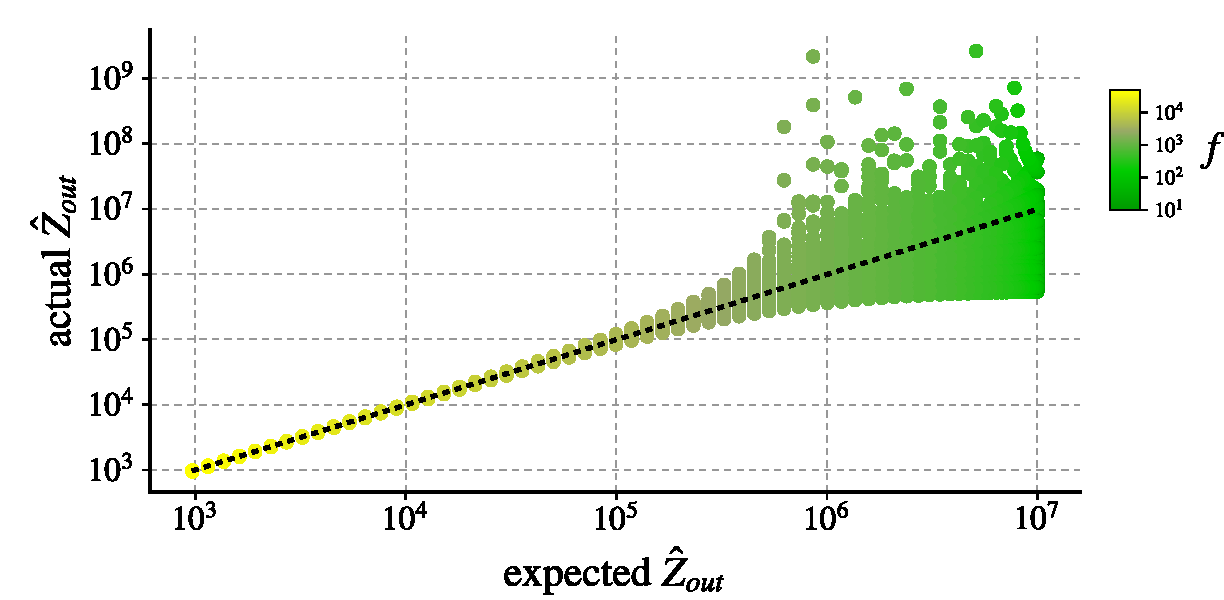
\includegraphics[scale=.6]{sensitivity_[method=voltage].pdf}
        % \caption{\small abc}
        \caption{}
        \label{fig:measurement_sensitivity_voltage}
    \end{subfigure}

	\begin{subfigure}{\textwidth}
        \centering
		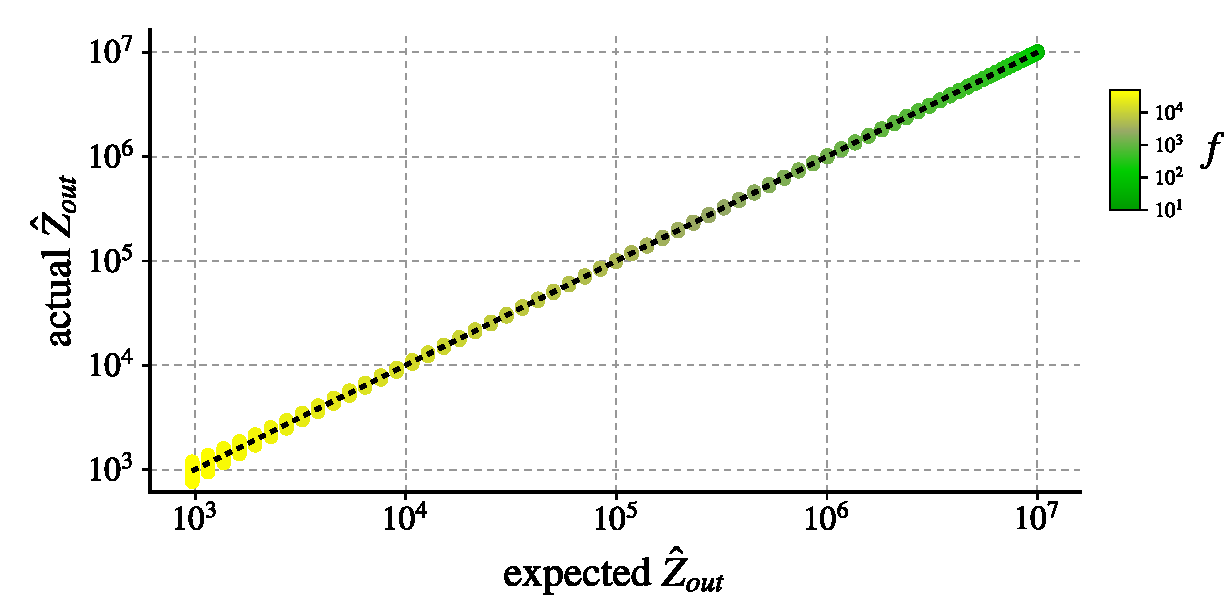
\includegraphics[scale=.6]{sensitivity_[method=current].pdf}
        \caption{}
        % \caption{\small}
        \label{fig:measurement_sensitivity_current}
    \end{subfigure}

\caption{\small Sensitivity of the measured $\hat{Z}_{out}$ to tolerance of the probe resistors $R_{L,a}$ and $R_{L,b}$, for voltage-based method (top) and current-based method (bottom). For each point, colour indicates the frequency at which it was measured; impedance drops at higher frequencies due to the presence of $C_{out}$.}
\label{fig:measurement_sensitivity}
\end{figure}
This expression is substituted into \briefeqlink{eq:z_out_quasi_volt}, yielding a theoretical prediction for $\hat{Z}_{out}$ as a function of frequency, parameterised by $R_{out}$ and $C_{out}$. The resulting curves exhibit a typical RC lowpass filter shape, with plateau and roll-off (see solid lines in \brieffiglink{fig:output_resistance_empirical} for examples).

%%%%%%%%%%%%%%%%%%%%%%%%%%%%%%%%%%%%%%%%%%%%%%%%%%%%%%%%%%%%%%%%%%%%%%%%%%%%%%
\subsubsection{Effects of probe resistor tolerance}
\label{sec:probe_resistor_effects}

Measurement artefacts may be introduced as a consequence of tolerance in the component values of $R_{L,a}$ and $R_{L,b}$. For example, at DC, let $R_{L,a}=10~\kilo\ohm.$ If $R_{L,b}$ is assumed to be $11~\kilo\ohm$, but its actual in-circuit value is $15~\ohm$ larger, then a $1~\mega\ohm$ output resistance will be reported as $2.8~\mega\ohm$ by the voltage-based method (a relative error of 280\%), but as $0.985~\mega\ohm$ by the current-based method (a relative error of only 1.5\%).

To quantify the artefact magnitude across frequency $f$, we sample values for $R_{L,a}$ and $R_{L,b}$ from a uniform distribution, centered upon a mean of $10~\kilo\ohm$ resp. $11~\kilo\ohm$, and within a 0.1\% tolerance range. An output capacitance of $1~\nano\farad$ is assumed. We compute an ``expected'' $\hat{Z}_{out}$, on the basis of ideal load resistors, and an ``actual'' $\hat{Z}_{out}$, based on the samples. The actual value (vertical axis) is then plotted with respect to the expected value (horizontal axis). If the measurement were completely insensitive to tolerance in the resistors, the actual value would be precisely the same as the expected value, causing all points to fall exactly on the diagonal, indicated by the dashed black lines in \brieffiglink{fig:measurement_sensitivity}. Any vertical offset between a point and the diagonal corresponds to the measurement artefact introduced by tolerance in the probe resistors.

The voltage-based method (\brieffiglink{fig:measurement_sensitivity}, top panel) is most sensitive to variations in probe resistor values there where it matters most: in the region of highest output impedance. This makes it an unsuitable method for measuring the output impedance of a current source, which is generally characterised by high output impedance. The current-based method (\brieffiglink{fig:measurement_sensitivity}, bottom panel) also suffers from sensitivity to probe resistance, but this occurs at higher frequency and consequently at values of $\hat{Z}_{out}$ that are so low as to be outside the range of interest for a VCCS.


%%%%%%%%%%%%%%%%%%%%%%%%%%%%%%%%%%%%%%%%%%%%%%%%%%%%%%%%%%%%%%%%%%%%%%%%%%%%%%
\subsection{SPICE simulation of output impedance}
\label{sec:spice_output_resistance}

We used \textsc{LTspice} \cite{ltspice} to simulate the three circuits, and calculate complex output impedance by \briefeqlink{eq:z_out_curr}. An op-amp model was used that characterises the op-amp by a few key parameters (\briefseclink{sec:op_amp_model}), listed in \tablelink{tbl:op_amp_parameters}. Model parameter values were chosen to match real-world values in order of magnitude. Some parameters were ignored or assumed infinite (e.g. maximum output current, slew rate).

\begin{table}[b!]
\centering
\bgroup
\def\arraystretch{1.3}%  1 is the default, change whatever you need
\newcolumntype{a}{>{\hsize=4\hsize}X}
\newcolumntype{b}{>{\hsize=13\hsize}X}
\newcolumntype{c}{>{\hsize=5.5\hsize}X}
\begin{tabularx}{.95\textwidth}{ a|b|c|c }
\specialcell{Symbol \\\ } & \specialcell{Name \\\ } & \specialcell{Value \\ (LT1211)} & \specialcell{Value\\ (simulation)} \\
\hline
\cellcolor{gray!4} $A_{OL}$ & \cellcolor{gray!4} open-loop gain & \cellcolor{gray!4} $1200~\volt/\milli\volt$ & \cellcolor{gray!4} $1000~\volt/\milli\volt$ \\
\cellcolor{gray!8} $GBW$ & \cellcolor{gray!8} gain-bandwidth product & \cellcolor{gray!8} $14~\mega\hertz$ & \cellcolor{gray!8} $10~\mega\hertz$ \\
\cellcolor{gray!4} $SR$ & \cellcolor{gray!4} slew rate & \cellcolor{gray!4} $7~\volt/\micro\second$ & \cellcolor{gray!4} $\infty$ \\
\cellcolor{gray!8} $R_{in}$ & \cellcolor{gray!8} input resistance & \cellcolor{gray!8} $40~\mega\ohm$ & \cellcolor{gray!8} $100~\mega\ohm$ \\
\cellcolor{gray!4} $C_{in}$ & \cellcolor{gray!4} input capacitance & \cellcolor{gray!4} $10~\pico\farad$ & \cellcolor{gray!4} $10~\pico\farad$ \\
\cellcolor{gray!8} $R_{out}$ & \cellcolor{gray!8} output resistance & \cellcolor{gray!8} $75~\ohm$ & \cellcolor{gray!8} $10~\ohm$ \\
% \cellcolor{gray!4} $CMRR$ & \cellcolor{gray!4} common-mode rejection ratio & \cellcolor{gray!4} $86~\decibel$ & \cellcolor{gray!4} \\
\cellcolor{gray!4} $PM$ & \cellcolor{gray!4} phase margin & \cellcolor{gray!4} $60\degree$ & \cellcolor{gray!4} \ang{55} \\
% \cellcolor{gray!8} $f_{p2}$ & \cellcolor{gray!8} frequency of second pole & \cellcolor{gray!8} & \cellcolor{gray!8} $3~\mega\hertz$ \\
\end{tabularx}\egroup
\caption{Op-amp parameters used for all \textsc{LTspice} simulations, unless stated otherwise. Values pertaining to the LT1211 were extracted from the datasheet \cite{LT1211_datasheet}.}
\label{tbl:op_amp_parameters}
\end{table}

Results are shown in \brieffiglink{fig:spice_ac_output_resistance}. Below $1~\mega\hertz$, the differential VCCS outperforms the single-ended version by a factor of 2. This is in line with the results of the Monte Carlo simulation.

Note that there is a tradeoff between output impedance and VCCS gain: in general, increasing the gain (by picking different resistor values) yields a lower (worse) $|R_{out}|$, and vice versa. For example, if the gain of the differential (but not the single-ended) VCCS is doubled (by picking its $R_{2b}=R_{4b}=500~\ohm$ and re-dimensioning remaining resistors to satisfy the conditions in \briefeqlink{eq:diff_howland_conditions}), then it will achieve the same $R_{out}$ as the single-ended version, across all frequencies and for all conditions shown in \brieffiglink{fig:spice_ac_output_resistance}.

\begin{figure}[t!]
	\begin{subfigure}{\textwidth}
        \centering
 		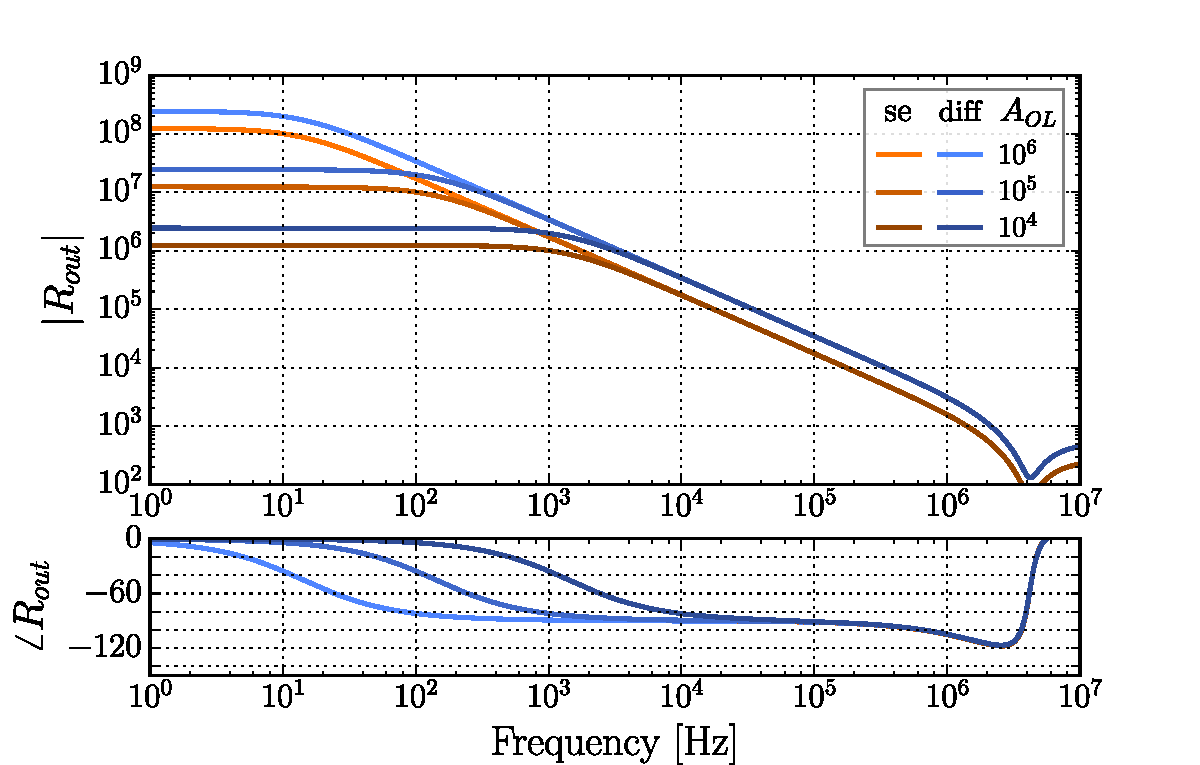
\includegraphics[scale=.6]{R_out_across_A_OL.pdf}
        \caption{\small }
        \label{fig:spice_ac_output_resistance_vs_AOL}
    \end{subfigure}

	\begin{subfigure}{\textwidth}
        \centering
 		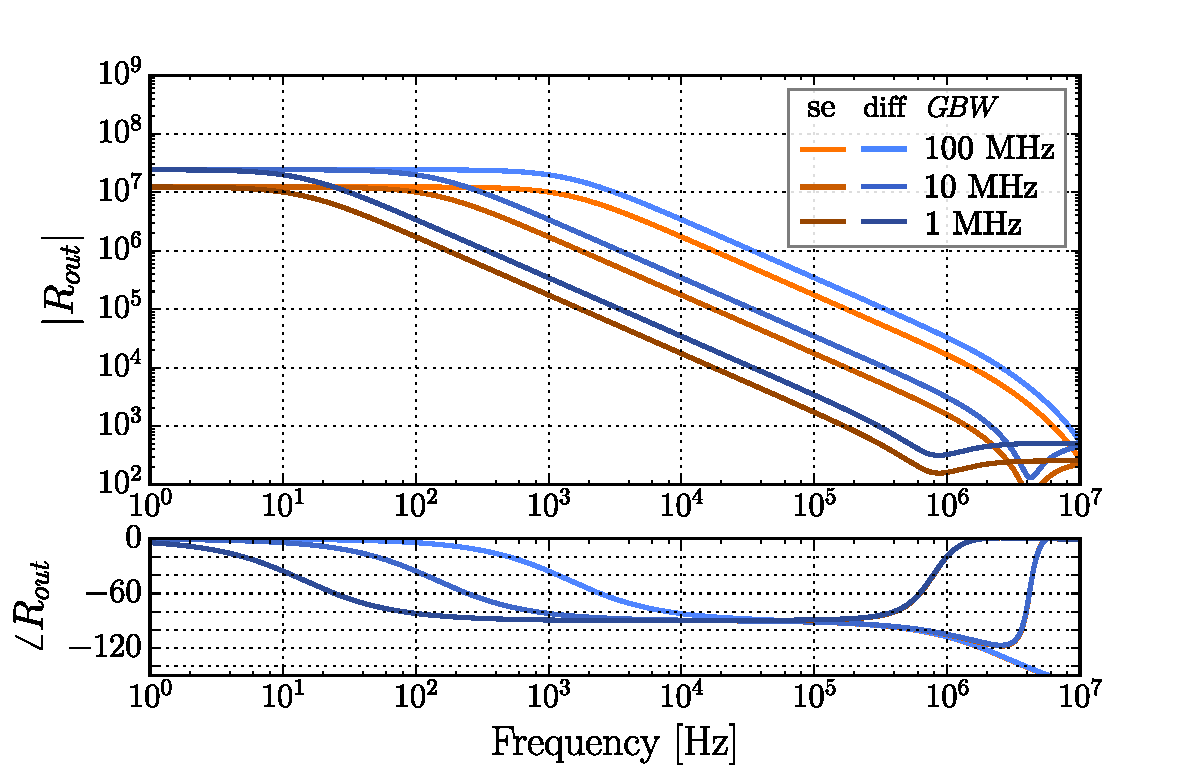
\includegraphics[scale=.6]{R_out_across_GBW.pdf}
        \caption{\small}
        \label{fig:spice_ac_output_resistance_vs_GBW}
    \end{subfigure}

    \caption{\small Output impedance (plotted as magnitude $|R_{out}|$ and phase $\OldAngle R_{out}$) of the single-ended (``se'') and differential (``diff'') VCCS. \textsc{LTspice} simulation. \textbf{Top:} parameter sweep across op amp open-loop gain $A_{OL}$ (between $10~\volt/\milli\volt$ and $1000~\volt/\milli\volt$). \textbf{Bottom:} parameter sweep across op amp gain-bandwidth product $GBW$ (between $1~\mega\hertz$ and $100~\mega\hertz$).}
    \label{fig:spice_ac_output_resistance}

\end{figure}

\begin{figure}[t!]
	\begin{subfigure}{\textwidth}
        \centering
		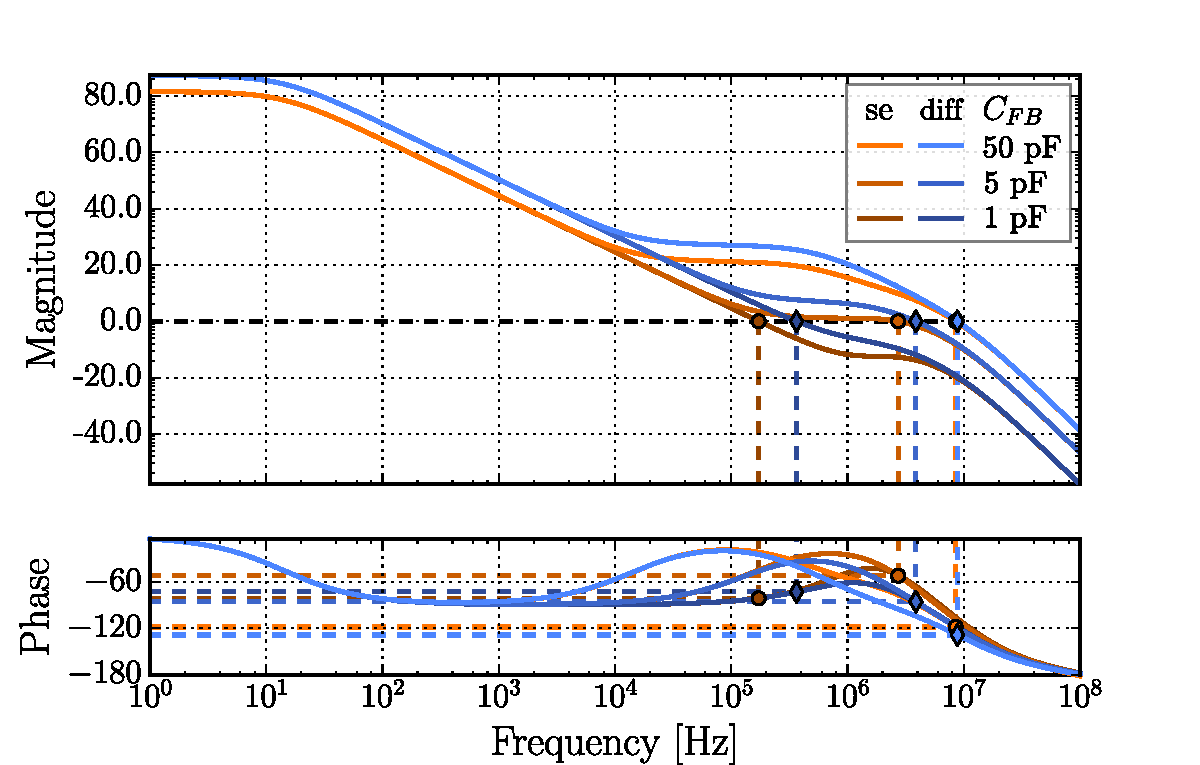
\includegraphics[scale=.6]{sim_phase_margins_resistive.pdf}
        % \caption{\small abc}
        \label{fig:phase_margins_resistive_load}
    \end{subfigure}

	\begin{subfigure}{\textwidth}
        \centering
		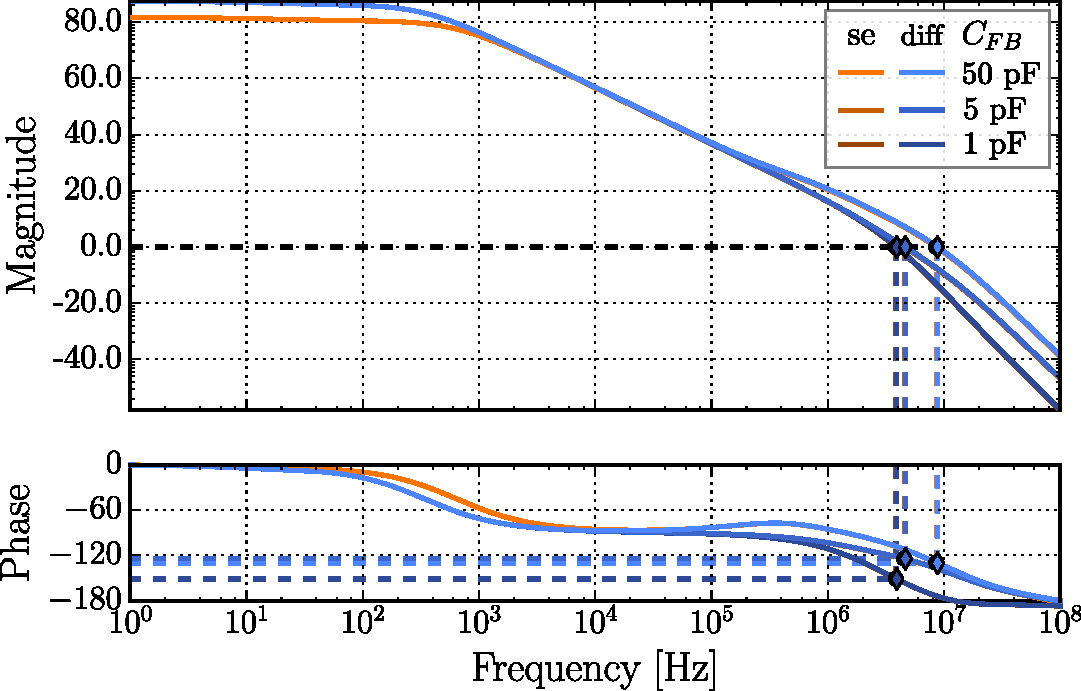
\includegraphics[scale=.6]{sim_phase_margins_capacitive.pdf}
        % \caption{\small}
        \label{fig:phase_margins_capacitive_load}
    \end{subfigure}

    \caption{\small Loop gain of the single-ended (``se'') and differential (``diff'') VCCS. \textbf{Top:} purely resistive load ($R_L=10~\kilo\ohm$). \textbf{Bottom:} capacitive load ($Z_L=10~\kilo\ohm\|1~\micro\farad$). Dashed lines indicate the method for reading off phase margin (see main text for details).}
    \label{fig:loop_gains_phase_margins}
\end{figure}



%%%%%%%%%%%%%%%%%%%%%%%%%%%%%%%%%%%%%%%%%%%%%%%%%%%%%%%%%%%%%%%%%%%%%%%%%%%%%%
\subsection{Loop stability and compensation}
\label{sec:loop_stability_compensation}

%%%%%%%%%%%%%%%%%%%%%%%%%%%%%%%%%%%%%%%%%%%%%%%%%%%%%%%%%%%%%%%%%%%%%%%%%%%%%%
\subsubsection{Preliminaries}

Loop stability refers to the propensity of the VCCS to oscillate, overshoot or  otherwise respond poorly to transients in load impedance or input voltage. A medical or research setting where a human subject is connected to the VCCS places very high demands on stability. At the same time, the human subject presents a challenging load. In circuit terms, interfaces between the electrodes and skin, as well as biological processes in the living tissue, yield a potentially very large capacitive effect, the magnitude of which depends on current frequency and amplitude \cite{lyklema_fundamentals}\cite{Grant2010}\cite{bioimpedance_bioelectricity}. Furthermore, when DC stimulation is applied, galvanic processes can occur \cite{lyklema_fundamentals} that change the electrical properties of the interface as a function of stimulation parameters such as current direction (cathodic vs. anodic) and amplitude. These processes are typically highly nonlinear. An ideal VCCS will remain stable under all load conditions.

Loop stability is often expressed in terms of \emph{phase margin}, which refers to the following oscillation criterion for any feedback circuit: the loop gain has to have a magnitude of 1 and a phase shift of $\ang{360}$ in order for the circuit to (potentially) oscillate. The phase margin, then, is defined as the difference between the actual loop phase and $\ang{360}$, at the frequency where the loop gain equals $0~\decibel$. A typical minimum acceptable phase margin is $\ang{60}$, with a higher number indicating better stability. The relationship between phase margin and time-domain phenomena such as overshoot and ringing are only well-defined for second-order systems, and become an approximation for higher order systems. We therefore validate the frequency-domain simulations with time-domain transient simulations (\briefseclink{sec:time_domain_transient_validation}).


%%%%%%%%%%%%%%%%%%%%%%%%%%%%%%%%%%%%%%%%%%%%%%%%%%%%%%%%%%%%%%%%%%%%%%%%%%%%%%
\subsubsection{`Lead' compensation method}

Lead compensation introduces a zero into the transfer function of the feedback circuit. Typically, the op-amp is modeled by means of two poles, each of which introduces $90\degree$ of phase lag. The zero due to the compensation circuit is then placed near the highest pole, cancelling part of the lag---hence the name lead compensation. Lead compensation is simple (it introduces only one extra parameter in the circuit) but considerably reduces the circuit bandwidth.

In the single-ended VCCS, lead compensation is implemented by placing a feedback capacitor $C_{FB}$ parallel to $R_2$ (see \brieffiglink{fig:single_ended_howland}). In the differential VCCS, two feedback capacitors $C_{FB,1}=C_{FB,2}=C_{FB}$ are placed in parallel with $R_1$ and $R_3$, respectively (see \brieffiglink{fig:differential_howland}).


%%%%%%%%%%%%%%%%%%%%%%%%%%%%%%%%%%%%%%%%%%%%%%%%%%%%%%%%%%%%%%%%%%%%%%%%%%%%%%
\subsubsection{Simulation method}

To evaluate the performance of the VCCS circuits with and without compensation, we use the Middlebrook method in \textsc{LTspice}. Briefly, this involves alternately inserting a voltage source and a current source into the feedback loop, each with a very small AC magnitude, so as to not disturb the DC setpoint of the circuit. The Middlebrook technique maintains a closed loop, thereby minimally disturbing normal circuit operation. The purpose of the inserted sources is to probe the response of the circuit to the injected voltages and currents. For this purpose, voltages and currents are measured on all ports of the inserted sources. The loop gain can then be derived by means of a simple algebraic expression \cite{middlebrook_method}.

For differential-output VCCS, we are interested in the differential-mode loop response, and use two ideal baluns \cite{kundert_balun} to convert between balanced and unbalanced signals. The baluns are inserted back-to-back at the place where we wish to insert the Middlebrook sources; here, immediately following the output of each op-amp. The first balun converts the balanced VCCS output to an unbalanced output, i.e. a separate differential-mode and a common-mode path. Middlebrook sources are then inserted into the differential path, and a second balun converts back to balanced output.


%%%%%%%%%%%%%%%%%%%%%%%%%%%%%%%%%%%%%%%%%%%%%%%%%%%%%%%%%%%%%%%%%%%%%%%%%%%%%%
\subsubsection{Simulation results: loop gain}

To understand how lead compensation affects stability, we run our simulations with a range of values for $C_{FB}$ between $1$ and $100~\pico\farad$. Additionally, to study the effect of different load conditions, the load capacitance $C_L$ is made to vary between $0$ (purely resistive load) and $1~\micro\farad$. Load capacitance is presented in parallel with a constant $10~\kilo\ohm$ resistor, so that $Z_L= C_L\|R_L$.

In \brieffiglink{fig:loop_gains_phase_margins}, the simulated loop gain is plotted in terms of magnitude and phase, for two load conditions (top panel: purely resistive; bottom panel: $C_L=1~\micro\farad$). The method for reading off phase margin (of the circuit, not the op-amp property) is indicated by dashed lines: first, find the frequency at which the loop gain magnitude equals one (black horizontal line). At this frequency, read off the loop gain phase (horizontal coloured lines); the phase margin $PM$ is then $\ang{-180}$ minus this number. Intersections are marked for convenience (circles: single-ended; diamonds: differential).

At DC, the loop gain of the differential supply is twice that of the single-ended supply ($\approx87$ and $81~\deci\bel$, respectively). We note that this will, generally speaking, make compensation easier for the single-ended supply, because lower gain tends to shift the $0~\deci\bel$ point to lower frequencies, where, in the absence of compensation, the phase margin is larger.%as demonstrated by the superior phase margin of the single-ended supply with respect to the differential version in the top panel and under the conditions $C_{FB}=5$ and $50~\pico\farad$.

The two lowest-frequency poles of the op-amp are responsible for two inflection points around $10~\hertz$ and $10~\mega\hertz$. The effect of increasing $C_{FB}$ is seen as an increase in the $0~\deci\bel$-frequency, and an associated boost in phase. Adding a substantial load capacitance (bottom panel) worsens the phase margins across the board, as expected. The obtained phase margins indicate that under some conditions, the differential VCCS outperforms the single-ended supply, whereas in other conditions, the situation might be reversed.%We note that other parameters not shown (in particular, $A_{OL}$ and $GBW$) further affect 

In general, we wish to pick the optimal $C_{FB}$, that leads to the best (highest) $PM$. The existence of a particular ``optimal'' $C_{FB}$ is suggested by the non-monotonic relationship between $C_{FB}$ and $PM$ (see e.g.` \brieffiglink{fig:loop_gains_phase_margins}, bottom panel: the best $PM$ is achieved by the intermediate value of the feedback capacitor).

\begin{figure}[t!]
        \centering
        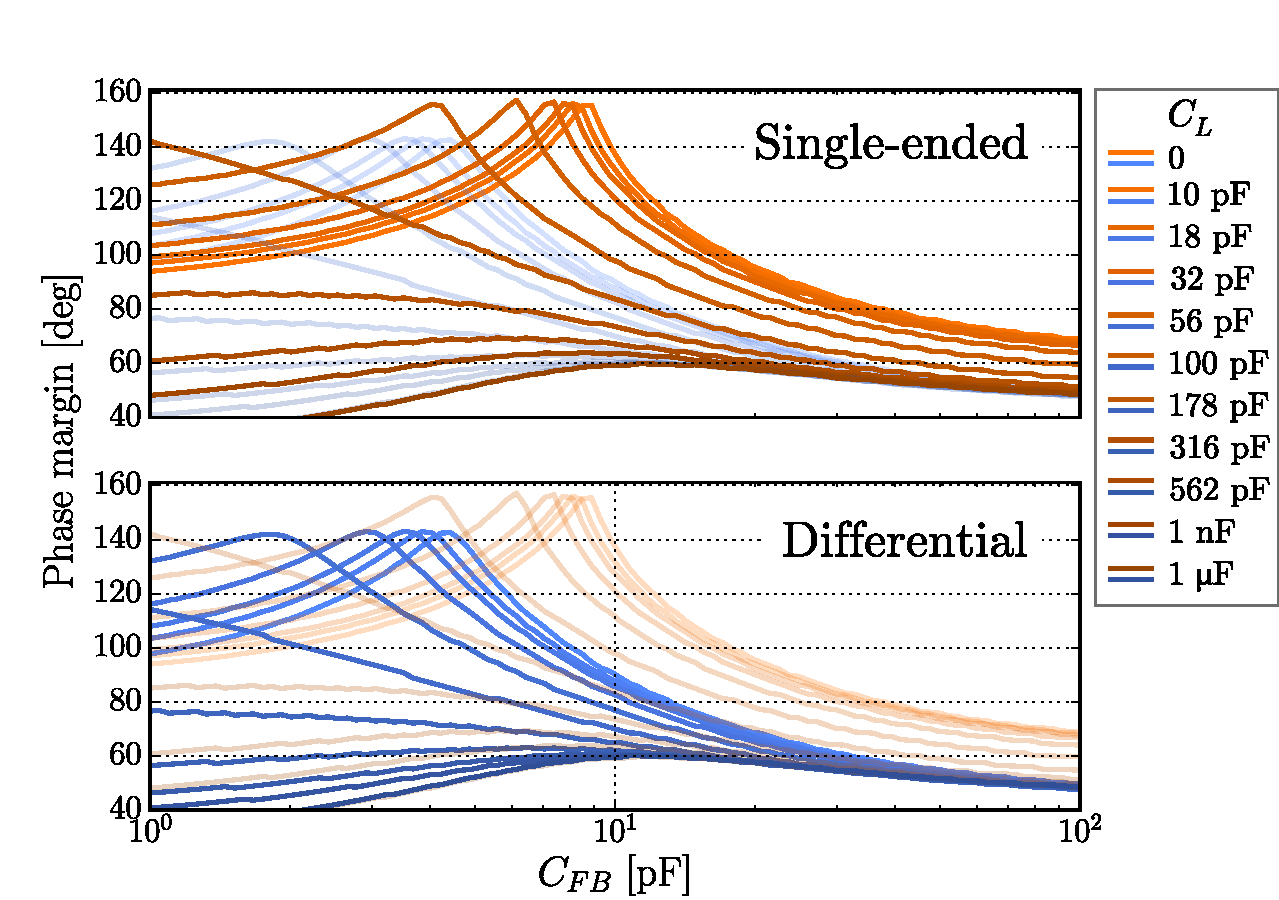
\includegraphics[scale=.6]{sim_phase_margins.pdf}
        \caption{\small Phase margin (PM) obtained for an op-amp with parameters as given in \tablelink{tbl:op_amp_parameters}, with the exception of $GBW=5~\mega\hertz$. To find the optimal $C_{FB}$, we simulate the PM for various loading conditions: $R_L$ is a constant $10~\kilo\ohm$, while $C_L$ varies between zero and $1~\micro\farad$. The optimal $C_{FB}$ can then be read from the diagram by finding the point on the horizontal axis where the PM is maximal.}
        \label{fig:phase_margins}
\end{figure}

To investigate this relationship in more detail, we performed a parameter sweep across $C_{FB}$ and plotted the phase margin obtained in each case (\brieffiglink{fig:phase_margins}). These curves indeed show a clear optimum, which for the differential supply occurs at approximately half the capacitance compared to the single-ended supply. For the same op-amp parameters and load, the differential supply can thus achieve a higher bandwidth. As the load capacitance increases, however, the optima of both circuits converge to approximately $10~\pico\farad$.% To account for the worst-case load condition, it is prudent to use this value in both circuits.

\begin{figure}[tb]
	\centering
	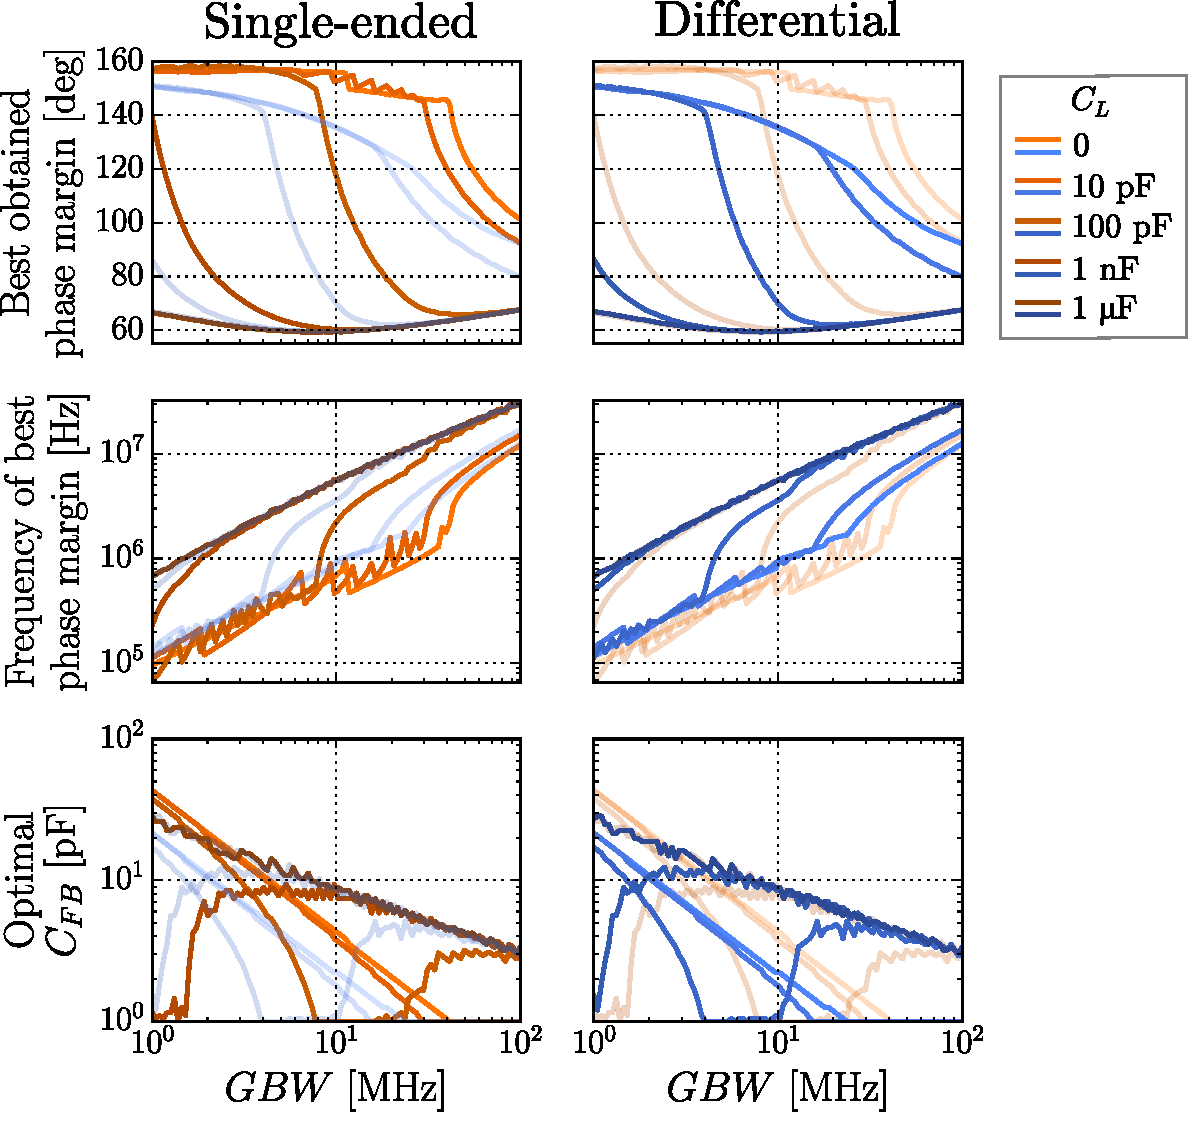
\includegraphics[scale=.6]{sim_phase_margins_vs_gbw_and_C_L.pdf}
	\caption{\small Phase margins versus the op-amp GBW parameter, for various values of $C_L$.}
	\label{fig:pm_vs_gbw_for_various_c_l}
\end{figure}

The plots in \brieffiglink{fig:phase_margins} were made for a fixed $GBW$. To better understand the relationship between $GBW$ and phase margin, we perform peak detection to identify the optimal $C_{FB}$ for each loading condition in \brieffiglink{fig:phase_margins}. We then sweep $GBW$ and plot, again for various load conditions, the best system performance that can be achieved (i.e. by picking the optimal $C_{FB}$).

Results are shown in \brieffiglink{fig:pm_vs_gbw_for_various_c_l}. The general trend is that a higher $GBW$ increases the frequency of the best achieved phase margin, and decreases the optimal $C_{FB}$. A higher VCCS bandwidth can thus indeed be achieved by picking an op-amp with higher $GBW$. Loop stability, however, suffers, as the achieved phase margins tend to be lower for higher $GBW$. It is thus in general easier to achieve stable operation for lower $GBW$, especially in the face of capacitive loading. For loads where the capacitance does not dominate the resistance, the differential supply outperforms the single-ended supply by offering more bandwidth.


%%%%%%%%%%%%%%%%%%%%%%%%%%%%%%%%%%%%%%%%%%%%%%%%%%%%%%%%%%%%%%%%%%%%%%%%%%%%%%
\subsubsection{Time-domain transient validation}
\label{sec:time_domain_transient_validation}

Predictions on the basis of loop gain should always be validated by time-domain transient testing. The transient should, ideally, not perturb the DC setpoint of the circuit. We apply a small-signal pulse to $V_{in,diff}$ so that a step occurs from $0.2475~\volt$ to $0.25~\volt$, corresponding to a change in requested current from $0.99~\milli\ampere$ to $1~\milli\ampere$. The corresponding transient in actual delivered output current is simultaneously measured, and inspected for signs of overshoot and ringing.

The transient response test is performed for a range of load capacitance values between zero and $1~\micro\farad$. As before, the load capacitor is in parallel with a load resistor of $10~\kilo\ohm$. All op-amp parameters are as in \brieftbllink{tbl:op_amp_parameters}. Under these conditions, we can read off the optimal $C_{FB}$ from the bottom two panels in \brieffiglink{fig:pm_vs_gbw_for_various_c_l} as $9~\pico\farad$ in both cases (single-ended and differential). We round the value to the nearest whole number, befitting the magnitude of numerical noise (e.g. discretisation errors, finite sweep resolution). According to formulas \briefeqlink{eq:single_ended_howland_transfer_function} and \briefeqlink{eq:diff_howland_transfer_function}, this places the $-3~\deci\bel$ point around $80~\kilo\hertz$ for both circuits under resistive load, well above the maximum frequencies typically used in tES.

The time-domain response is shown in \brieffiglink{fig:transient_response_sim} (left panel). The output current magnitude exhibits considerable overshoot for the differential, but not the single-ended circuit, in spite of the compensation. The underlying cause is the imbalance in driving impedance between the op-amp inverting and noninverting inputs. In the differential circuit, the non-inverting op-amp inputs are both driven by ideal voltage sources, whereas the inverting inputs are connected to the rest of the circuit via resistors on the order of $10~\kilo\ohm$. Combined with stray capacitance at the op-amp inputs, this results in a low-pass RC filter for the inverting but not the non-inverting inputs.

To compensate for this effect, we add a $10~\kilo\ohm$ resistor in series with each non-inverting input. The right panel of \brieffiglink{fig:transient_response_sim} shows that the inclusion of these resistors indeed eliminates the overshoot. Note that the steady-state curves for single-ended and differential circuits no longer precisely overlap, indicating a slight DC offset due to the interaction between the added resistors and the finite input resistance at each op-amp input (here, $10~\mega\ohm$; see \brieftbllink{tbl:op_amp_parameters}).

\begin{figure}[tb]
	\centering
    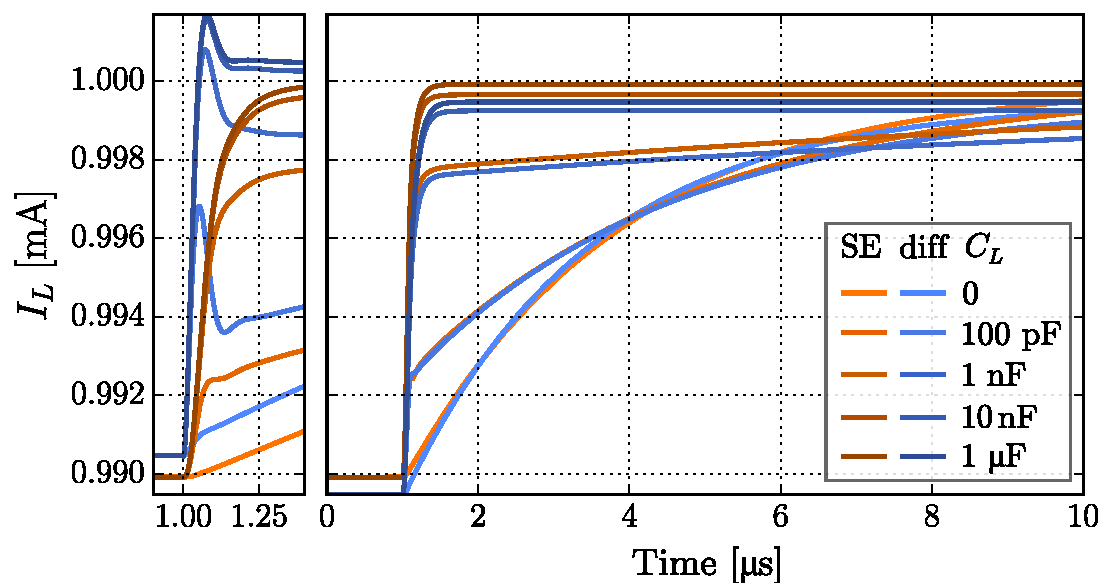
\includegraphics[scale=.6]{transient_response.pdf}
	\caption{\small Transient response to a step function at $t=1~\micro\second$ corresponding to a change in requested current from $0.99~\milli\ampere$ to $1~\milli\ampere$. The trend is that higher load capacitance leads to a faster response in actual delivered current. \textbf{Left:} detailed view showing overshoot and ringing (mostly) for the differential but not the single-ended VCCS, in the case that no extra precautions are taken. \textbf{Right:} overview of response demonstrating that additional input resistors eliminate the overshoot (see discussion in \briefseclink{sec:time_domain_transient_validation}).}
	\label{fig:transient_response_sim}
\end{figure}


%%%%%%%%%%%%%%%%%%%%%%%%%%%%%%%%%%%%%%%%%%%%%%%%%%%%%%%%%%%%%%%%%%%%%%%%%%%%%%
\subsubsection{Out-of-the-loop compensation method}
\label{sec:out_of_loop_compensation}

Initial simulations showed that the best achieved phase margin at the most demanding loading condition is below the minimum acceptable. A simple and robust way to improve $PM$ is to isolate the VCCS from capacitive loading by inserting one (for single-ended) or two resistors (for differential) in series with the load. These resistors are inserted between the output terminal(s) of the VCCS and the load.

The downside of this method is that we incur an extra (Ohmic) voltage drop. As an example, say that we pick a value of $100~\ohm$ for the series resistors. The voltage drop will be $0.5~$and $1~\volt$ for the single-ended and differential supplies, respectively, at the maximum output current $I_L=5~\milli\ampere$. The phase margin is considerably improved, by approximately $\ang{15}$, and is achieved at a lower value of $C_{FB}$, thereby improving bandwidth. These series resistors were not included in any of the reported results, but their inclusion in the final tES application circuit is strongly recommended to provide an additional safety margin.



%%%%%%%%%%%%%%%%%%%%%%%%%%%%%%%%%%%%%%%%%%%%%%%%%%%%%%%%%%%%%%%%%%%%%%%%%%%%%%%
%%%%%%%%%%%%%%%%%%%%%%%%%%%%%%%%%%%%%%%%%%%%%%%%%%%%%%%%%%%%%%%%%%%%%%%%%%%%%%%
\section{Empirical results}
\label{sec:empirical-results}

%%%%%%%%%%%%%%%%%%%%%%%%%%%%%%%%%%%%%%%%%%%%%%%%%%%%%%%%%%%%%%%%%%%%%%%%%%%%%%
\subsection{Description of the prototypes}
\label{sec:description_of_the_prototype}

Two prototype circuits were built to validate predictions from theory and simulation with empirical measurements. Circuits were constructed using surface-mount devices in SOIC-8 and 1206 ($3.2\times1.6~\milli\meter$) packages on a 1.6 mm dual layer FR-4 PCB with a ground plane on the bottom layer. Devices were battery-powered with a linearly regulated bipolar supply of $\pm15~\volt$.

%%%%%%%%%%%%%%%%%%%%%%%%%%%%%%%%%%%%%%%%%%%%%%%%%%%%%%%%%%%%%%%%%%%%%%%%%%%%%%
\subsubsection{Component selection}

Selection criteria for the op-amp include wide output voltage swing, high current drive capability, a high gain-bandwidth product and otherwise excellent characteristics (offset voltages and currents, distortion, noise, etc.) The op-amp used in the prototypes is the Linear Technology LT1211 (dual op-amp in a SOIC-8 package) \cite{LT1211_datasheet}. In the single-ended circuit, the second op-amp in the package is not used, and is wired as a voltage follower with its noninverting input tied to ground. This was done in order to obtain the best possible match between the testing conditions of each circuit.

All fixed resistors used in the circuit were rated at a tolerance of $0.1\%$. Some of the resistors were implemented as the series connection of a fixed resistance and a potentiometer to allow for trimming (see \briefseclink{sec:trimming}). The $250~\ohm$ fixed resistors were implemented as the parallel connection of a $300~\ohm$ and $1.5~\kilo\ohm$ resistor. The $10.25~\kilo\ohm$ fixed resistors were implemented as the parallel connection of two $20.5~\kilo\ohm$ resistors.

Feedback capacitors were picked according to the methods of \briefseclink{sec:loop_stability_compensation}. When the parameters of the LT1211 are entered, the optimum values returned by the simulation are approximately $5.5~\pico\farad$ for the single-ended, and $3.0~\pico\farad$ for the differential circuit. We round these to the standard component values of $C_{FB}=3.3~\pico\farad$ (for the differential circuit) and $C_{FB}=6.6~\pico\farad$ (for the single-ended circuit: implemented as the parallel connection of two $3.3~\pico\farad$ capacitors).


%%%%%%%%%%%%%%%%%%%%%%%%%%%%%%%%%%%%%%%%%%%%%%%%%%%%%%%%%%%%%%%%%%%%%%%%%%%%%%
\subsubsection{Input drive signal}

The inputs of each VCCS were driven in antiphase, such that $V_{in,neg}=-V_{in,pos}$ at all times.

Note that the single-ended VCCS presents a more demanding load to the circuit driving its input terminals, because the input driver needs to supply the nonzero current that flows through resistors $R_1$ and $R_3$. The output impedance of the driver appears in series with these (precision) resistors and can cause \briefeqlink{eq:single_ended_howland_conditions} to be violated. For this reason, an additional dual op-amp (LT1211) was used in the single-ended VCCS as a unity gain input buffer. Numerical simulation confirmed that the impact of the buffer on the overall AC response of the (combined) circuit is negligible. The differential VCCS does not present the disadvantage of needing an additional input buffer; its input impedance is already very high, equal to twice the impedance at the noninverting op-amp input.

\begin{figure}[t!]
\begin{subfigure}{\textwidth}
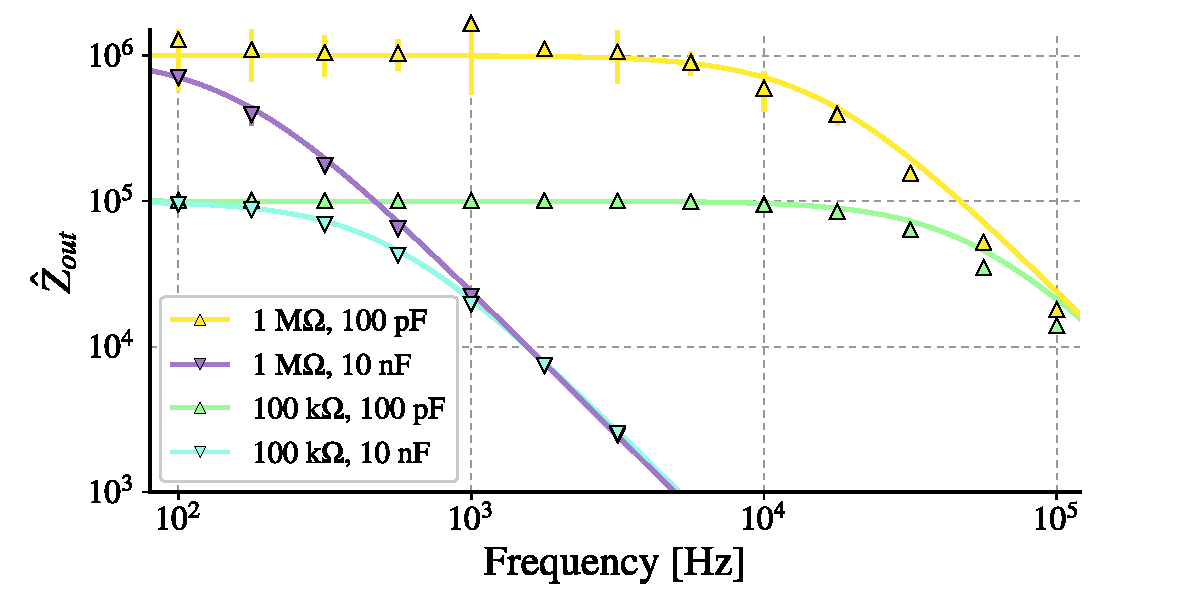
\includegraphics[scale=.6]{../paper/output_resistance_empirical_ref.pdf}
\caption*{}
\end{subfigure}
\ \\
\begin{subfigure}{\textwidth}
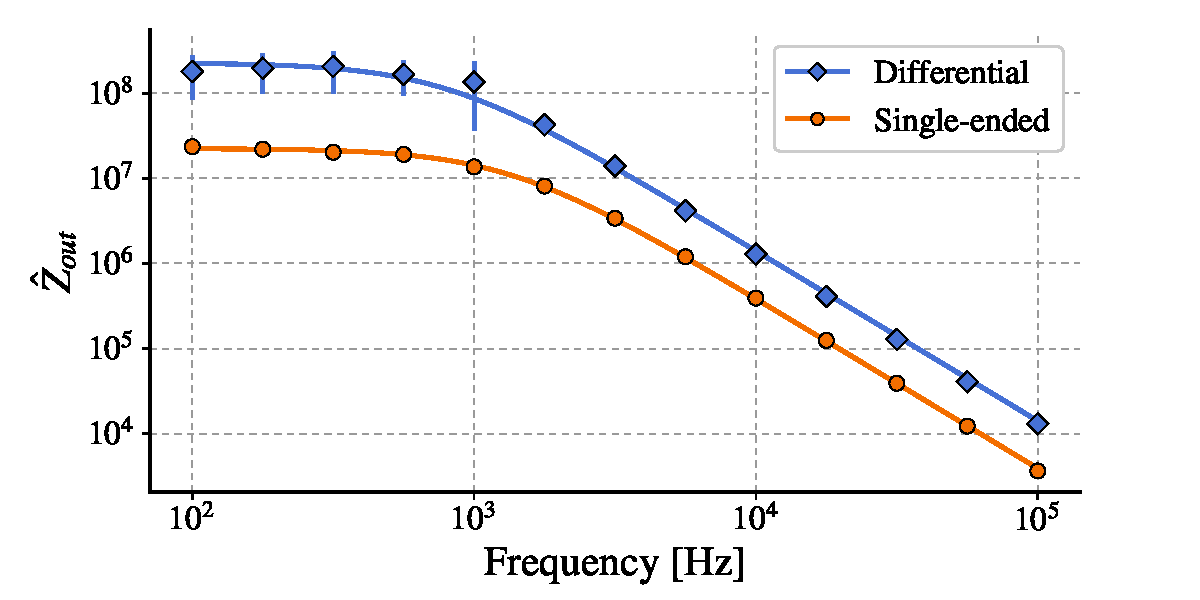
\includegraphics[scale=.6]{../paper/fig_output_resistance_empirical.pdf}
\caption*{}
\end{subfigure}
\caption{\small Empirical output resistance measurements for reference loads (top panel) and single-ended and differential VCCS circuits (bottom panel). Error bars due to measurement noise are plotted for each datapoint, but are visible only for the highest impedances.}
\label{fig:output_resistance_empirical}
\end{figure}

%%%%%%%%%%%%%%%%%%%%%%%%%%%%%%%%%%%%%%%%%%%%%%%%%%%%%%%%%%%%%%%%%%%%%%%%%%%%%%
\subsubsection{Measuring output current}

To measure actual delivered current, an instrumentation amplifier (INA128U, Texas Instruments, USA) was set up to measure voltage drop across a $10~\ohm$ resistor $R_{sens}$ placed in series with the load (\brieffiglink{fig:impedance_measurement_method}). The instrumentation amplifier was configured for a gain of 51, so a current of 1 mA yields a measured voltage of 0.51 V. For a 6-digit multimeter, this in turn yields a maximum theoretical measurable output impedance of $510~\mega\ohm$. Higher gain will improve the highest measurable impedance, but reduces the highest measurable frequency (here, 100 kHz) due to the finite gain-bandwidth product of the instrumentation amplifier.


%%%%%%%%%%%%%%%%%%%%%%%%%%%%%%%%%%%%%%%%%%%%%%%%%%%%%%%%%%%%%%%%%%%%%%%%%%%%%%
\subsection{Trimming procedure}
\label{sec:trimming}

To trim output resistance, $R_2$ in the single-ended, and $R_1$ and $R_3$ in the differential circuit were implemented as the series connection of a fixed resistor and a trimmer potentiometer. Trimming was performed as follows. The VCCS was set for a DC current of $1~\milli\ampere$. Two loads were alternately applied to the source: a short circuit, and a $10~\kilo\ohm$ resistor. The actual delivered current was measured, and the trimmer potentiometer was adjusted until these values converged. For the differential source, the trimming potentiometers were alternately adjusted in small increments until covergence.

All reported values throughout this paper were obtained using the same, fixed trim.


%%%%%%%%%%%%%%%%%%%%%%%%%%%%%%%%%%%%%%%%%%%%%%%%%%%%%%%%%%%%%%%%%%%%%%%%%%%%%%
\subsection{Measurement of output impedance}
\label{sec:empirical_output_resistance}

To measure output impedance, the current-based method (\briefeqlink{eq:z_out_quasi_curr}) was used as described in \briefseclink{sec:output_impedance_measurement}. Resistor values $R_{L,a}=10~\kilo\ohm$ and $R_{L,b}=11~\kilo\ohm$ were selected to obtain an output voltage close to the compliance voltage, and for having a relatively small difference between them while taking finite measurement precision into account. 

A Hewlett-Packard 33120A function generator generates the input drive signal $V_{in,diff}$. To convert the single-ended output voltage into a differential voltage for driving the VCCS, a battery-powered unity gain buffer using a fully differential output op-amp was used.

A Hewlett-Packard 3456A 6-digit digital voltmeter was used for data acquisition. Samples were acquired at a rate of $1~\hertz$ via GPIB interface on a GNU/Linux host computer. The voltmeter was connected to the output of an instrumentation amplifier as described in \briefseclink{sec:description_of_the_prototype} to acquire readings for $I_L$. Samples which resulted in $\hat{Z}_{out}=\infty$ were discarded. This setup allowed us to reliably measure output resistance up to about $100~\mega\ohm$ (see variance bars in \brieffiglink{fig:output_resistance_empirical}).

The function generator and voltmeter were set up for automated data acquisition via the IEEE~488 (``GPIB'') instrument bus. To allow easy switching between load resistances, $R_L$ was implemented as the series connection of a $10~\kilo\ohm$ and $1~\kilo\ohm$ resistor, both with a tolerance of $0.1\%$, and a relay that short-circuits the $1~\kilo\ohm$ resistor when activated.

The method was first validated using a reference circuit with known values. A function generator (sinusoidal voltage source) with $50~\ohm$ output impedance was connected in series with a resistor of known value: $100~\kilo\ohm$ or $1~\mega\ohm$. This is the Th\'{e}venin equivalent of a current source with an output resistance of the same value. Simultaneously, this ``current source'' was loaded with a load capacitance $C_L=100~\pico\farad$ or $10~\nano\farad$, simulating the output capacitance $C_{out}$. This ``current source'' was then characterised using the same method. Results are shown in the top panel of \brieffiglink{fig:output_resistance_empirical}. In this figure, empirical data is represented as points, while predicted values, based on the known $R_{out}$ and $C_{out}$, are plotted as solid lines. The limit of voltmeter resolution is especially visible in the $1~\mega\ohm$ condition, due to the large Ohmic voltage drop resulting in a very small load current. Overall, a good match between the empirical data and theoretical predictions can be observed, validating the accuracy and precision of our methodology.

\begin{table}[t!]
\centering
\bgroup
\def\arraystretch{1.3}%  1 is the default, change whatever you need
\newcolumntype{a}{>{\hsize=4\hsize}X}
\newcolumntype{b}{>{\hsize=13\hsize}X}
\newcolumntype{c}{>{\hsize=5.5\hsize}X}
\begin{tabularx}{5.7cm}{ a|c|c }
 & Single-ended & Differential\\
\hline
$R_{out}$ & $22.5~\mega\ohm$ & $249~\mega\ohm$ \\
$C_{out}$ & $245~\pico\farad$ & $131~\pico\farad$ \\
\end{tabularx}\egroup
\caption{\small Fitted values for resistive and capacitive components of the output impedance.}
\label{tbl:Z_hat_out_curve_fit}
\end{table}

Next, the VCCS prototypes were characterised. The bottom panel of \brieffiglink{fig:output_resistance_empirical} shows both the empirical measurements (as points), and the theoretical prediction based on curve fitting (as solid lines). To perform curve fitting, the Nelder-Mead algorithm \cite{neldermead} was used to find the $R_{out}$ and $C_{out}$ that minimise an error measure, defined as the squared difference between the (base 10) logarithm of the predicted, and logarithm of the empirical $\hat{Z}_{out}(f)$, summed over all measured frequencies $f$. Fitting was done independently for each circuit. Overall, good agreement between empirical data and the fitted curves is observed in \brieffiglink{fig:output_resistance_empirical}, supporting the resistive-capacitive model of VCCS output impedance. Results of the fit are repeated in \brieftbllink{tbl:Z_hat_out_curve_fit} to allow a more precise quantitative comparison. The DC output resistance of the differential source is seen to outperform the single-ended source by a factor of more than 2, exceeding the improvement that was predicted based on theory in \briefseclink{sec:monte_carlo}. Because we trim each circuit towards the singularity point where $R_{out}$ approaches infinity, sensitivity to trim near this point is extremely high, explaining the variance. In contrast, the capacitive part of the output impedance $C_{out}$ comes much closer to a factor 2 improvement from the single-ended to the differential circuit. This can be attributed to the high-frequency behaviour being dominated by the $C_{FB}$ capacitors, which were chosen a factor of 2 different in value.

%%%%%%%%%%%%%%%%%%%%%%%%%%%%%%%%%%%%%%%%%%%%%%%%%%%%%%%%%%%%%%%%%%%%%%%%%%%%%%
\subsection{Transfer function and bandwidth}

\begin{figure}[t!]
	\centering
    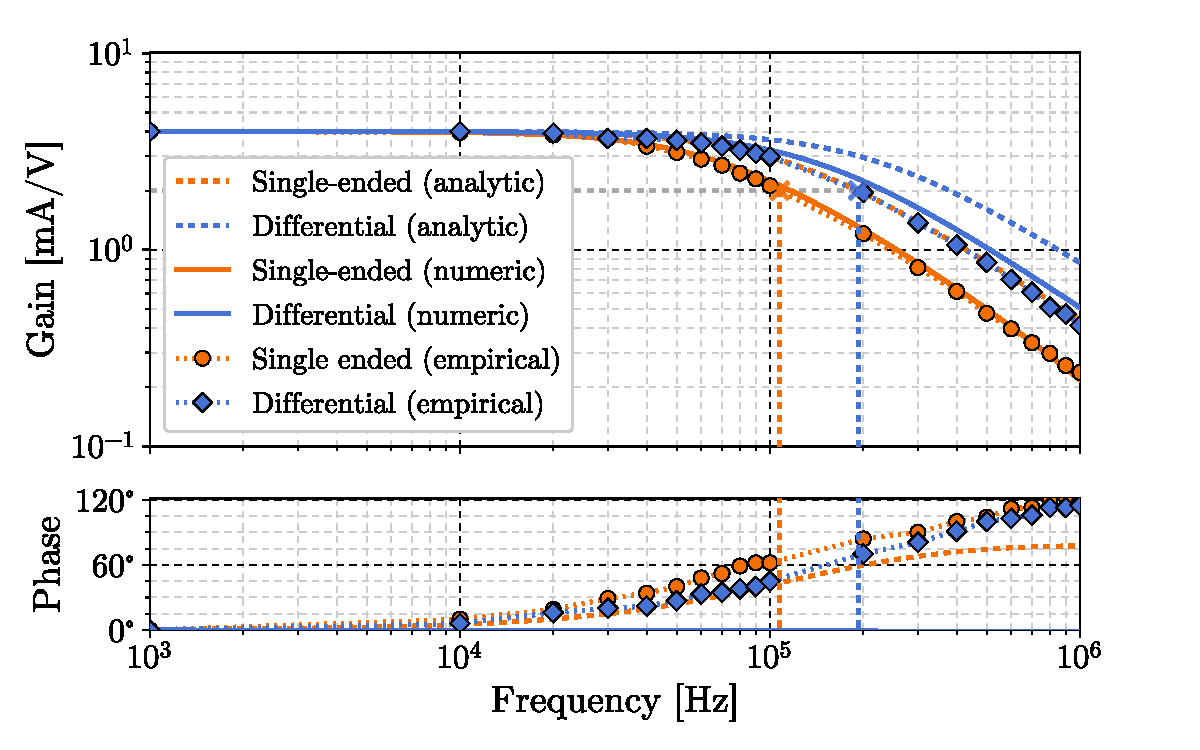
\includegraphics[scale=.6]{transfer_function.pdf}
	\caption{\small Bode plot. $R_L=10~\kilo\ohm$}
	\label{fig:bode_plot}
\end{figure}

The transfer function (\brieffiglink{fig:bode_plot}) is plotted on the basis of three data sources for comparison: the analytic formulas (\briefeqlink{eq:single_ended_howland_transfer_function}, \briefeqlink{eq:diff_howland_transfer_function}), numeric (\textsc{LTspice}) simulation, and empirical data. Simulations were run using the op-amp parameters in \brieftbllink{tbl:op_amp_parameters}; differences caused by switching to the built-in \textsc{LTspice} LT1211 model were negligible. Note that the analytic formulas assume an ideal op-amp and consequently overestimate the frequency response. When an ideal op-amp is used in simulation, the analytic curves overlap precisely with the numeric curves.

Overall, the data shows a factor two improvement in cutoff frequency in the differential VCCS compared to the single-ended version. This corresponds to the choice of a $C_{FB}$ twice as high for the single-ended circuit compared the differential circuit (see \briefseclink{sec:description_of_the_prototype}). We additionally verified the factor two improvement in marginally stable circuits with $C_{FB}=0$ (data not shown).



%%%%%%%%%%%%%%%%%%%%%%%%%%%%%%%%%%%%%%%%%%%%%%%%%%%%%%%%%%%%%%%%%%%%%%%%%%%%%%
\subsection{Harmonic distortion}

The output spectra were measured while applying a sinusoidal input voltage at $100~\hertz$ to $V_{in,diff}$, such that $I_{L,peak}=1~\milli\ampere$. The actual delivered current was measured at the output of one of the instrumentation amplifiers, acquired for 300 seconds, and saved as a 32 bit float uncompressed wave file. After windowing with a 4-term Blackman-Harris window, the Fourier transform of the signal was obtained and normalised to precisely $1~\milli\ampere$ at $100~\hertz$.

If the output of a nonlinear system, such as a non-ideal VCCS, is differential rather than single-ended, all even harmonic terms (at even multiples of $100~\hertz$) cancel out. The second harmonic (at $200~\hertz$) was indeed found to be approximately $6~\deci\bel$ smaller in the differential than in the single-ended circuit (\brieffiglink{fig:output_current_spectrum}). The third harmonic (odd, at $300~\hertz$) and higher harmonics are also visible, and appear of approximately equal magnitude in both circuits.

The total harmonic distortion (THD) of an amplifier is defined as a magnitude ratio between the load current $I_{L,fund}$ at the fundamental, and the load current $I_{L,n}$ at each harmonic (for $n\geq 2$):

\begin{align*}
THD &= \frac{\sqrt{\left(\sum_{n=2}^\infty I_{L,n} \right)}}{I_{L,fund}}
\end{align*}

Data was acquired using a U24XL 24-bit USB DAC/ADC at a sampling rate of $48~\kilo\hertz$. Harmonics beyond the third are close to the noise floor of the experimental setup, and do not contribute significantly to the THD value (see \brieffiglink{fig:output_current_spectrum}). THD was therefore calculated based on the second and third harmonics (\brieftbllink{tbl:thd}). The differential supply improves over the single-ended circuit by a factor of more than three.

\begin{figure}[t!]
	\centering
    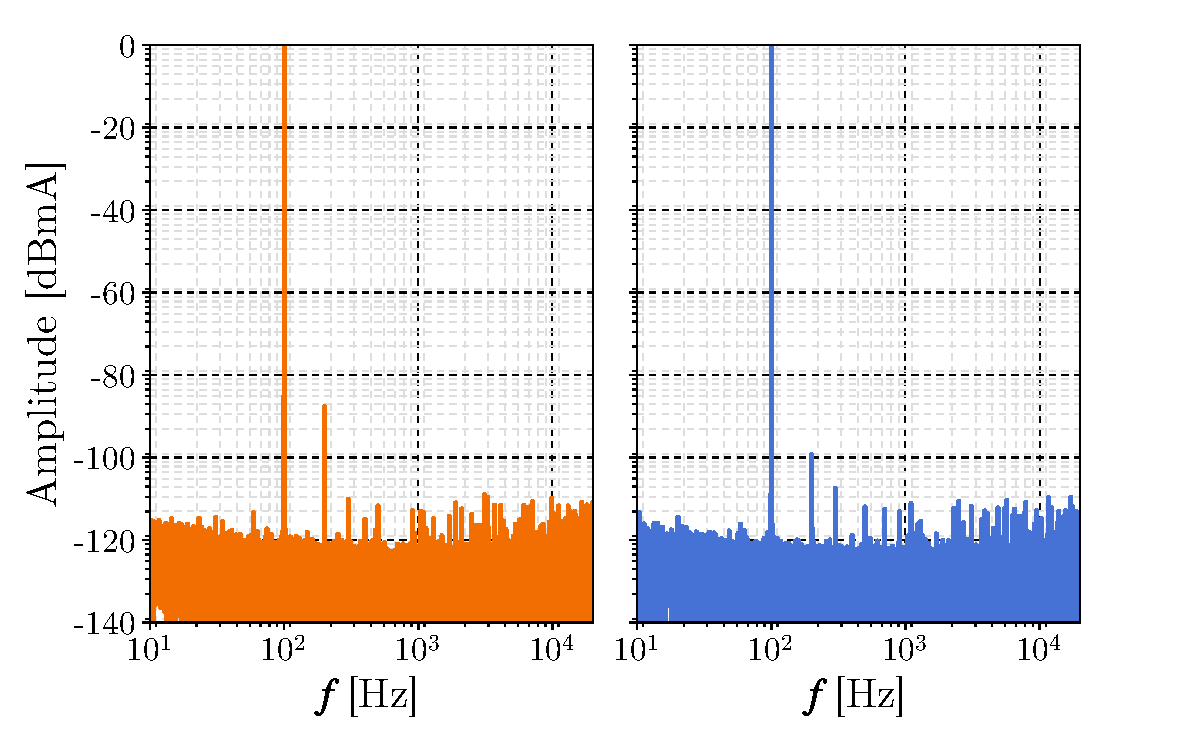
\includegraphics[scale=.6]{spectral_analysis.pdf}
	\caption{\small Spectrum of $I_L$ for for a $100~\hertz$ sine input at $V_{in,diff}$ such that $I_L=1~\milli\ampere$.}
	\label{fig:output_current_spectrum}
\end{figure}

\begin{table}[b!]
\centering
\bgroup
\def\arraystretch{1.3}
\newcolumntype{c}{>{\hsize=5.5\hsize}X}
\begin{tabularx}{.39\textwidth}{ c|c }
Single-ended & Differential  \\
\hline
\cellcolor{gray!4} $4.1\cdot{}10^{-5}$ & \cellcolor{gray!4} $1.2\cdot{}10^{-5}$ \\
\end{tabularx}\egroup
\caption{Total Harmonic Distortion (THD) based on second and third harmonics.}
\label{tbl:thd}
\end{table}


%%%%%%%%%%%%%%%%%%%%%%%%%%%%%%%%%%%%%%%%%%%%%%%%%%%%%%%%%%%%%%%%%%%%%%%%%%%%%%
\subsection{Common-mode rejection ratio (CMRR)}

Common-mode rejection ratio (CMRR) is a measure of the immunity of the VCCS to a signal that appears simultaneously on the positive and negative input terminals. % If the circuit driving these terminals (e.g. a digital-to-analog converter) is well designed, the common-mode component in this driving signal should be infinitessimal and CMRR of the VCCS is therefore not critical. However, we include CMRR measurements here for completeness.
To account for a CMRR less than infinity, an extra term is added to \briefeqlink{eq:diff_gain} to account for common-mode gain $A_{cm}$ in addition to the differential gain $A_d$ (corresponding to $A$ in the original equation):
\begin{equation}
I_L = A_d\cdot(V_{in,pos} - V_{in,neg}) + A_{cm}\cdot \frac{V_{in,pos} + V_{in,neg}}{2}
\end{equation}
The CMRR is then defined as (in units of decibel):
\begin{equation}
\text{CMRR} = 20\cdot\log_{10}\left(\frac{A_d}{|A_{cm}|}\right)
\end{equation}
A sinusoidal common-mode signal was applied to both positive and negative phase inputs, with an amplitude such that, if one of the inputs were shifted in phase by $\ang{180}$, the output current would be $I_L=1~\milli\ampere$ (peak).

The CMRR achieved was similar across circuits and across frequencies (\brieftbllink{tbl:cmrr}).




%%%%%%%%%%%%%%%%%%%%%%%%%%%%%%%%%%%%%%%%%%%%%%%%%%%%%%%%%%%%%%%%%%%%%%%%%%%%%%
\subsection{Input transient response}

To validate stability under real-world conditions, we performed a test using a square wave profile for the input voltage, corresponding to a current of $I_{L,peak}=1~\milli\ampere$ into a $10~\kilo\ohm$ load. Measurements show a stable response without overshoot or ringing (\brieffiglink{fig:transient_response}). Adding a capacitor in parallel to the load resistor causes faster fall and rise times in $I_L$, because the output voltage does not need to swing as high to achieve the same load current, but no overshoot or ringing was observed (data not shown).

\begin{figure}[b!]
	\centering
    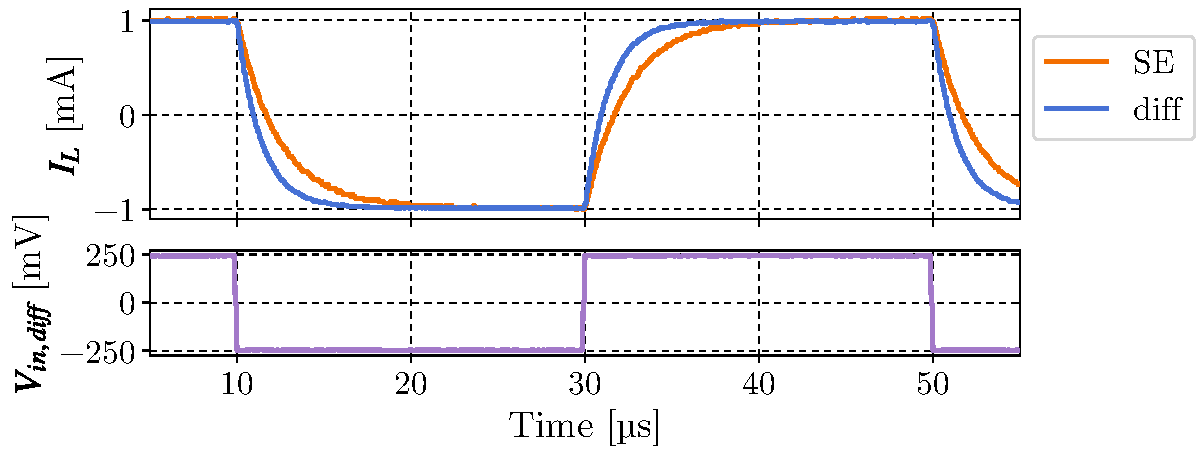
\includegraphics[scale=.6]{fig_transients.pdf}
	\caption{\small Transient response to a $f=25~\kilo\hertz$ square wave at $V_{in,diff}$ with a $10~\kilo\ohm$ resistive load.}
	\label{fig:transient_response}
\end{figure}

\begin{table}[t!]
\centering
\bgroup
\def\arraystretch{1.3}
\newcolumntype{a}{>{\hsize=4\hsize}X}
\newcolumntype{c}{>{\hsize=5.5\hsize}X}
\begin{tabularx}{.54\textwidth}{ a|c|c }
$f$ & Single-ended & Differential \\
\hline
\cellcolor{gray!4} $100~\hertz$ & \cellcolor{gray!4} $54~\deci\bel$ & \cellcolor{gray!4} $53~\deci\bel$ \\
\cellcolor{gray!8} $10~\kilo\hertz$ & \cellcolor{gray!8} $51~\deci\bel$ & \cellcolor{gray!8} $53~\deci\bel$ \\
\end{tabularx}\egroup
\caption{Common-mode rejection ratio achieved by each VCCS, at two tested frequencies.}
\label{tbl:cmrr}
\end{table}


%%%%%%%%%%%%%%%%%%%%%%%%%%%%%%%%%%%%%%%%%%%%%%%%%%%%%%%%%%%%%%%%%%%%%%%%%%%%%%
\subsection{Load transient response}

A second transient test was carried out to evaluate VCCS stability, by changing the load resistance while the input voltage $V_{in,diff}$ was kept constant, corresponding to $I_L=1~\milli\ampere$. A $10~\kilo\ohm$ resistor was used as load, while a second $100~\ohm$ resistor was electrically inserted and removed, in parallel with the other resistor. The electrical switching was carried out by driving an opto-isolator (International Rectifier PVT412S \cite{PVT412_datasheet}) with a square wave input and placing it series with the second resistor. When the opto-isolater is switched off (for low $V_{ctrl}$, see lower panel of \brieffiglink{fig:load_transient_response}), the total load resistance is $10~\kilo\ohm$, whereas for high $V_{ctrl}$, the load resistance drops to approximately $100~\ohm$. These resistances were chosen so that the output voltage spans the full scale from $V_L=10~\volt$ to almost zero (\brieffiglink{fig:load_transient_response}, middle panel).

A step change in load resistance requires a step change in output voltage to maintain the same current. Because the voltage cannot change instantaneously, a momentary transient is observed in actual delivered output current (\brieffiglink{fig:load_transient_response}, top panel). When the load resistance decreases, the voltage is momentarily too low (for the given input voltage) and a transient undercurrent occurs around $t=300~\micro\second$. The delay between the change in $V_{ctrl}$ (at $t=100~\micro\second$) and the first observable response (around $t=275~\micro\second$) can be attributed to turn-off delay of the opto-coupler \cite{PVT412_datasheet} (and likewise for the turn-on delay starting at $t=600~\micro\second$).The differential VCCS shows a roughly twofold improvement over the single-ended supply.

\begin{figure}[t!]
	\centering
    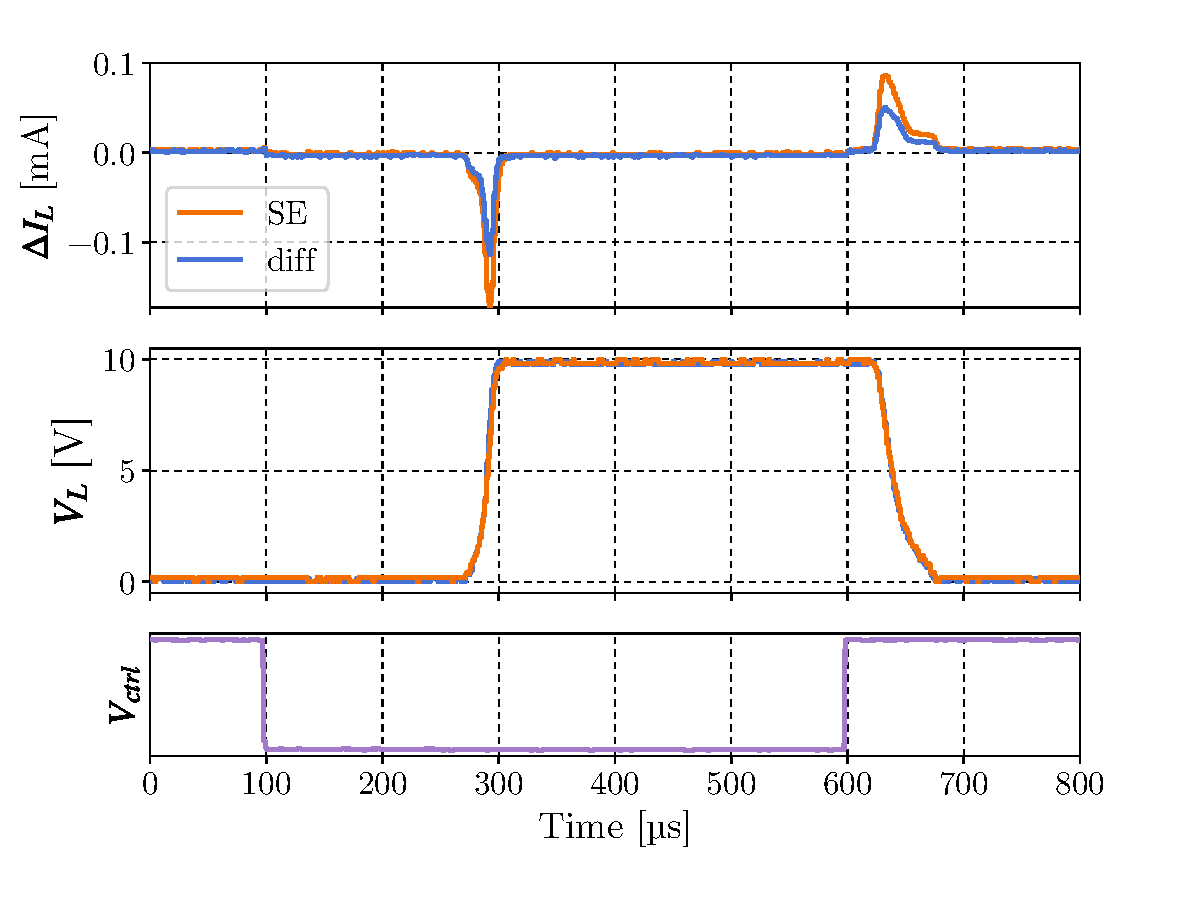
\includegraphics[scale=.6]{fig_load_transient.pdf}
	\caption{\small Transient response to a change in load resistance. Load resistance was alternated between $10~\kilo\ohm$ ($V_{ctrl}$ low) and $100~\ohm$ ($V_{ctrl}$ high).}
	\label{fig:load_transient_response}
\end{figure}



\subsection{Temperature sensitivity}
%%%%%%%%%%%%%%%%%%%%%%%%%%%%%%%%%%%%%%%

\begin{figure}[b!]
        \centering
        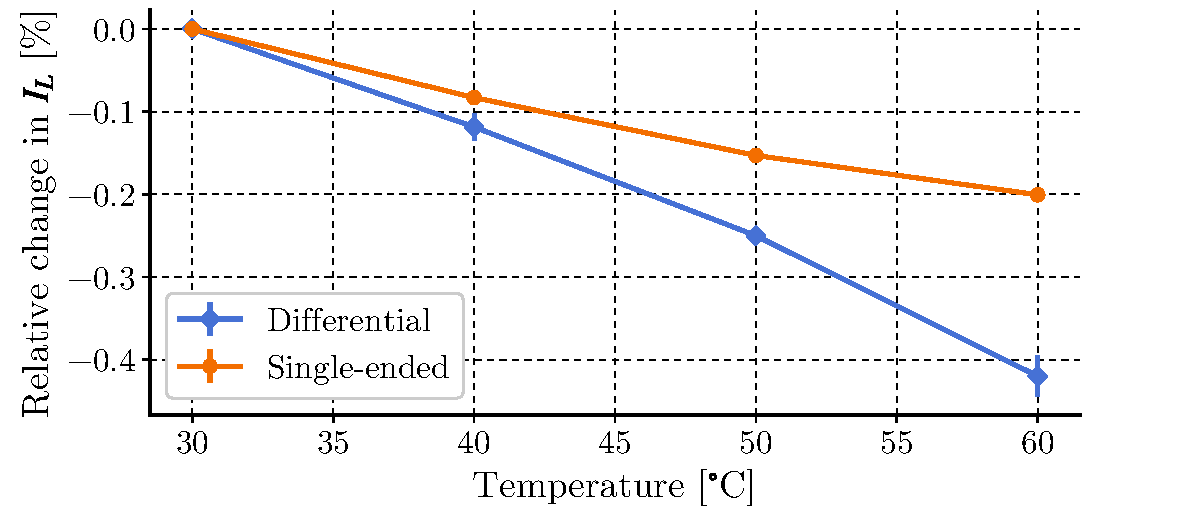
\includegraphics[scale=.6]{fig_temperature_coeff.pdf}
        \caption{\small Temperature dependence of output current for a given input voltage. The temperature dependence was measured relative to a $1~\milli\ampere$ current into a $10~\kilo\ohm$ load at $30~\celsius$. Error bars indicate standard deviation over 5 heating/cooling cycles.}
        \label{fig:temp_coeff}
\end{figure}

Thermal drift is an undesirable property of a VCCS, where, in spite of a constant $V_{in,diff}$, the actual delivered current changes as a function of temperature.

The prototype, including the single-ended input buffer and current measuring instrumentation amplifiers, but not the load resistor, was heated from \SI{30}{\celsius} up to \SI{60}{\celsius}, while the actual current delivered was measured for a setlevel corresponding to $I_L=1~\milli\ampere$ at the lowest temperature. All resistors used in the prototype have a temperature coefficient of $25~\text{ppm}$.

\textsc{LTspice} simulation with ideal op-amps, but $25~\text{ppm}$ resistors, suggests that the temperature coefficient of the single-ended and differential circuits should be almost indistuingishable. Empirical results instead show a temperature coefficient about twice as large for the differential compared to the single-ended circuit (\brieffiglink{fig:temp_coeff}). The difference is attributable to non-ideal op-amp behaviour, such as input bias currents that are a function of temperature \cite{LT1211_datasheet}.


%%%%%%%%%%%%%%%%%%%%%%%%%%%%%%%%%%%%%%%%%%%%%%%%%%%%%%%%%%%%%%%%%%%%%%%%%%%%%%
\section{Conclusion}
\label{sec:conclusion}
%%%%%%%%%%%%%%%%%%%%%%%%%%%%%%%%%%%%%%%%%%%%%%%%%%%%%%%%%%%%%%%%%%%%%%%%%%%%%%

On the basis of analysis and simulation, we conclude that only the current-based method for measuring VCCS output impedance has practical application value (\briefseclink{sec:probe_resistor_effects}). In addition, we find empirically that we can infer the full, complex-valued $Z_{out}$ on the basis of the proxy measurement of $\hat{Z}_{out}$ (\briefseclink{sec:proxy_output_impedance}). Our method is suitable for VCCS circuits with a fully differential output, and was able to provide reliable data up to about $100~\mega\ohm$ at frequencies up to $100~\kilo\hertz$.

The differential VCCS requires two potentiometers to be trimmed instead of one. Although the trimming process is relatively simple and only needs to be carried out once, we note that \cite{lee2003precision} use a digital potentiometer to automate the trimming process. The absence of resistors connected with one terminal to ground in the differential version complicates this method, but an analogous approach could in principle be used to avoid manual trimming.

In general, for electronics that is used \emph{in vivo} in medicine or research, an abundance of caution should be exercised. A higher voltage range should be used with care; depending on operating conditions, keeping the voltage low can contribute to safety \cite{pmid15661300}. Output impedance measurement of the VCCS should be complemented by time-domain transient validation, temperature stability testing, common-mode output voltage measurements, and so on. Additional safety margins (such as on loop stability), low-current fuses and other passive and active protection mechanisms are crucial steps in going from the core VCCS circuit to a ready-to-use, clinical or research tES device, and indicate potential directions for future research.


%%%%%%%%%%%%%%%%%%%%%%%%%%%%%%%%%%%%%%%%%%%%%%%%%%%%%%%%%%%%%%%%%%%%%%%%%%%%%%
%%%%%%%%%%%%%%%%%%%%%%%%%%%%%%%%%%%%%%%%%%%%%%%%%%%%%%%%%%%%%%%%%%%%%%%%%%%%%%
\appendix

%%%%%%%%%%%%%%%%%%%%%%%%%%%%%%%%%%%%%%%%%%%%%%%%%%%%%%%%%%%%%%%%%%%%%%%%%%%%%%
\section{Op-amp model}
\label{sec:op_amp_model}

We use a simple op-amp model with 7 parameters: input resistance $R_{in}$ and capacitance $C_{in}$, open-loop voltage gain $A_{OL}$, output resistance $R_{out}$, and three poles with frequencies $f_1, f_2$ and $f_3$ (\brieffiglink{fig:op_amp_model}).

We find it convenient to define the gain-bandwidth product $GBW$ as the frequency at which the open-loop op-amp gain equals 1. Most of the loss in gain at $GBW$ (compared to $A_{OL}$ at DC) is due to the first, low-frequency pole. We pick $f_2=GBW$, which means that the gain is reduced by an additional $3~\dB$ at GBW due to the second pole. It is then easy to calculate $f_1$ such that the overall gain equals 1 at $GBW$:
\begin{align}
\label{eq:gbw_pole_freq}
f_1 &= \frac{GBW}{\sqrt{\left(\frac{A_{OL}}{1.413}\right)^2 - 1}}
\end{align}
The constant 1.413 is equal to $-3~\deci\bel$ of voltage gain. Note that with this choice of pole frequencies, the phase margin of the op-amp is always $\ang{180}-\ang{135}=\ang{55}$, due to a $\ang{90}$ contribution of the first pole, and $\ang{45}$ from the second. The third pole is present in order to improve high-frequency rolloff, and we always choose $f_3 = 100\cdot{}GBW$.

Each pole stage $n$ (for $1\leq{}n\leq{}3$) is implemented by the parallel combination of a resistor and a capacitor (\brieffiglink{fig:op_amp_model}, dashed box). We pick $R_n=1~\kilo\ohm$ and calculate $C_n=1/(2\pi{}f_nR_n$). Each RC circuit is coupled to the previous stage by means of a voltage-controlled current source $g_n$ with gain $1/R_n$ and control voltage $V_{in,pos}-V_{in,neg}$ for the first stage, and $V_{n-1}$ for stage $n>1$.

The DC gain of the op-amp is modeled by the output buffer $E_{out}$, a voltage-controlled voltage source with gain $A_{OL}$, and control voltage that of the final pole stage $V_N$.


\begin{figure}
\centering
\makebox[\textwidth][c]{%
\begin{circuitikz}
	\node [label=left:$V_{in,pos}$] (Vinpos) at (-7, -1) {};
	\node [label=left:$V_{in,neg}$] (Vinneg) at (-7, 1) {};
	\node [] (op_vin_p) at (-5.5, -1) {};
	\node [] (op_vin_n) at (-5.5, 1) {};
	\node [] (op_vin_p2) at (-4, -1) {};
	\node [] (op_vin_n2) at (-4, 1) {};

	\draw (Vinneg.center) to [short, o-*] (op_vin_n.center) {};
	\draw (Vinpos.center) to [short, o-*] (op_vin_p.center) {};
	\draw (op_vin_p.center) to [R, l=$R_{in}$] (op_vin_n.center) {};

	\draw (op_vin_n.center) to [short] (op_vin_n2.center) {};
	\draw (op_vin_p.center) to [short] (op_vin_p2.center) {};
	\draw (op_vin_p2.center) to [C, l=$C_{in}$] (op_vin_n2.center) {};


	%
	% 	RC poles: box
	%

	\node [] (vboxtr) at (3, 2) {};
	\node [] (vboxbr) at (3, -2) {};
	\node [] (vboxtl) at (-3, 2) {};
	\node [] (vboxbl) at (-3, -2) {};

	\draw[dashed] (vboxtr.center) to [short] (vboxbr.center) {};
	\draw[dashed] (vboxbr.center) to [short] (vboxbl.center) {};
	\draw[dashed] (vboxbl.center) to [short] (vboxtl.center) {};
	\draw[dashed] (vboxtl.center) to [short] (vboxtr.center) {};



	%
	% 	RC poles
	%

	\node [] (gainshaping_gt) at (-1.5, 1) {};
	\node [] (gainshaping_gb) at (-1.5, -1) {};
	\node [label=above:$V_{n}$] (gainshaping_rt) at (0, 1) {};
	\node [] (gainshaping_rb) at (0, -1) {};
	\node [] (gainshaping_ct) at (1.5, 1) {};
	\node [] (gainshaping_cb) at (1.5, -1) {};
	\draw (gainshaping_gb.center) to [american controlled current source, l=$g_{n}$] (gainshaping_gt.center) {};
	\draw (gainshaping_gb.center) to [short, *-] ++(0, -.2) node [rground] {};
	\draw (gainshaping_rt.center) to [R, l=$R_{n}$, *-*] (gainshaping_rb.center) {};
	\draw (gainshaping_ct.center) to [C, l=$C_{n}$] (gainshaping_cb.center) {};
	\draw (gainshaping_gt.center) to [short] (gainshaping_rt.center) {};
	\draw (gainshaping_rt.center) to [short] (gainshaping_ct.center) {};
	\draw (gainshaping_gb.center) to [short] (gainshaping_rb.center) {};
	\draw (gainshaping_rb.center) to [short] (gainshaping_cb.center) {};


	%
	% 	the output VCVS and output resistance
	%

	\node [] (v1t) at (4, 1) {};
	\node [] (v1b) at (4, -1) {};
	\node [label=right:$V_{out}$] (f1bp) at (7, 1) {};
	\draw (v1t.center) to [american controlled voltage source, l=$E_{out}$] (v1b.center) {};
	\draw (v1t.center) to [R, l=$R_{out}$, -o] (f1bp.center) {};
	\draw (v1b.center) to [short] ++(0, -.2) node [rground] {};
\end{circuitikz}
}
\caption{\small Circuit model for op-amps used in the \textsc{LTspice} simulatons. The dashed box indicates a single pole stage and is replicated once for each pole in the model.}
\label{fig:op_amp_model}
\end{figure}


%%%%%%%%%%%%%%%%%%%%%%%%%%%%%%%%%%%%%%%%%%%%%%%%%%%%%%%%%%%%%%%%%%%%%%%%%%%%%%
\section{Repository}
\label{sec:repo}

All simulations, analysis and plotting scripts, prototype PCB designs and empirical measurement data, are available as supplementary material at:\\
\href{https://github.com/turingbirds/howland_vccs}{https://github.com/turingbirds/howland\_vccs}.

%%%%%%%%%%%%%%%%%%%%%%%%%%%%%%%%%%%%%%%%%%%%%%%%%%%%%%%%%%%%%%%%%%%%%%%%%%%%%%
\section{Citation}

This unabridged preprint, which was \colorbox{yellow!30}{not peer reviewed}, contains additional background information such as loop stability simulations, that could be helpful in reproducing and iterating upon the results in the paper published as\\[.5em]

\noindent
\begin{changemargin}{2em}{2em}
C. Linssen and P. Harpe, ``Practical Measurement of Voltage-Controlled Current Source Output Impedance for Applications in Transcranial Electrical Stimulation,'' 2021 IEEE Biomedical Circuits and Systems Conference (BioCAS), 6--9 Oct 2021, pp. 1-6,\href{https://doi.org/10.1109/BioCAS49922.2021.9644974}{doi: 10.1109/BioCAS49922.\\2021.9644974}.
\end{changemargin}

\noindent Please find the final accepted peer-reviewed paper in the repository (\briefappxlink{sec:repo}).


%%%%%%%%%%%%%%%%%%%%%%%%%%%%%%%%%%%%%%%

\renewcommand{\bibfont}{\small}
\setlength{\bibsep}{0mm}

\bibliographystyle{IEEEtran}
\bibliography{howland_vccs}

\end{document}

